%% Cleaned Beamer file converted to Metropolis
\documentclass[english,aspectratio=169]{beamer}

% -------------------------------------------------
% Fonts and encoding
% -------------------------------------------------
\usepackage[T1]{fontenc}
\usepackage[latin9]{inputenc}
\usepackage{lmodern}
\renewcommand{\sfdefault}{lmss}
\renewcommand{\ttdefault}{lmtt}

% -------------------------------------------------
% Language and layout
% -------------------------------------------------
\usepackage{babel}
\setlength{\parskip}{\medskipamount}
\setlength{\parindent}{0pt}

% -------------------------------------------------
% Math, graphics, listings
% -------------------------------------------------
\usepackage{amssymb}
\usepackage{graphicx}
\usepackage{color}
\usepackage{tikz}
\usepackage{listings}
\renewcommand{\lstlistingname}{Listing}
\usepackage{media9}   % modern package for embedding video

% -------------------------------------------------
% Theme: Metropolis
% -------------------------------------------------
\usetheme{metropolis}
\metroset{progressbar=frametitle,sectionpage=progressbar}

% -------------------------------------------------
% UCT Brand Colors
% -------------------------------------------------
\definecolor{UCTBlue}{HTML}{009ADA}
\definecolor{UCTDarkBlue}{HTML}{00243A}

\setbeamercolor{palette primary}{bg=UCTDarkBlue, fg=white}
\setbeamercolor{frametitle}{bg=UCTDarkBlue, fg=white}
\setbeamercolor{progress bar}{fg=UCTBlue}
\setbeamercolor{title separator}{fg=UCTBlue}
\setbeamercolor{alerted text}{fg=UCTBlue}

% -------------------------------------------------
% Custom UCT title slide
% -------------------------------------------------
\setbeamertemplate{title page}{%
  \begin{tikzpicture}[remember picture,overlay]
    % Background
    \fill[UCTBlue] (current page.south west) rectangle (current page.north east);
    % Logo
    \node[anchor=north, xshift=-4cm, yshift=-1.2cm] at (current page.north)
      {\includegraphics[height=1cm]{uct_logo_horizontal_white}};
    \node[anchor=north, xshift=4cm, yshift=0cm] at (current page.north)
      {
\includegraphics[height=3cm]{samos-logo-transparent}};      
  \end{tikzpicture}
  \vspace*{3.2cm}
  \begin{center}
    {\usebeamercolor[fg]{title}\usebeamerfont{title}\textcolor{white}{\inserttitle}}\\[0.6em]
    {\usebeamerfont{subtitle}\textcolor{white}{\insertsubtitle}}\\[1.2em]
    {\usebeamerfont{author}\textcolor{white}{\insertauthor}}\\[0.3em]
    {\usebeamerfont{institute}\textcolor{white}{\insertinstitute}}\\[0.8em]
    {\usebeamerfont{date}\textcolor{white}{\insertdate}}
  \end{center}
}

% -------------------------------------------------
% Footer logo for content slides
% -------------------------------------------------
\usepackage{tikzpagenodes}
\addtobeamertemplate{footline}{}{%
  \begin{tikzpicture}[remember picture,overlay]
    \node[anchor=south east, xshift=-1cm, yshift=0cm]
      at (current page.south east)
      {\includegraphics[height=0.5cm]{uct_logo_horizontal_blue}};
    \node[anchor=south west, xshift=0cm, yshift=-0.2cm]
      at (current page.south west)
      {
\includegraphics[height=0.7cm]{samos-logo-transparent.png}};  
  \end{tikzpicture}%
}

% -------------------------------------------------
% LyX-specific definitions (kept minimal)
% -------------------------------------------------
\makeatletter

\newcommand\makebeamertitle{\frame{\maketitle}}

\AtBeginDocument{%
  \let\origtableofcontents=\tableofcontents
  \def\tableofcontents{\@ifnextchar[{\origtableofcontents}{\gobbletableofcontents}}
  \def\gobbletableofcontents#1{\origtableofcontents}
}

\newenvironment{lyxcode}
  {\begin{list}{}{
     \setlength{\rightmargin}{\leftmargin}
     \setlength{\listparindent}{0pt}
     \setlength{\itemsep}{0pt}
     \setlength{\parsep}{0pt}
     \raggedright\normalfont\ttfamily
   }\item[]}
  {\end{list}}

\makeatother

% -------------------------------------------------
% Document
% -------------------------------------------------


\begin{document}

    \title[EC ]{Introduction to ocean modelling}
    \author{Marcello Vichi}
    \institute[UCT]{Department of Oceanography\\marcello.vichi@uct.ac.za}
    \date{AOS-SAMOS}
    \maketitle

\begin{frame}{Outline}
    \tableofcontents{}
\end{frame}


%-------------------------------------------------
\begin{frame}{Why do Ocean Scientists Need Models?}
\url{https://www.noc.ac.uk/discover-the-ocean/learning-hub/ocean-science-in-action/introduction-ocean-modelling-its-all-numbers}
\begin{itemize}
\item The ocean is constantly changing in space and time
\item Physical processes control:
\begin{itemize}
\item Nutrient supply
\item Plankton blooms
\item Oxygen and carbon cycles
\end{itemize}
\item Models help us:
\begin{itemize}
\item Understand processes
\item Fill observational gaps
\item Test hypotheses ("what if?")
\end{itemize}
\end{itemize}
\end{frame}

%-------------------------------------------------
\begin{frame}{What is a Model?}
\begin{block}{Definition}
A model is a simplified representation of reality used to describe and predict system behaviour.
\end{block}

\begin{itemize}
\item We select key variables (e.g. temperature, currents, nutrients)
\item We define the relationships between them
\item We simulate their evolution in time and space
\end{itemize}
\end{frame}

%-------------------------------------------------
\begin{frame}{The Barents Sea Model of the Norwegian Meteorological Institute}
    \begin{figure}
        \centering
        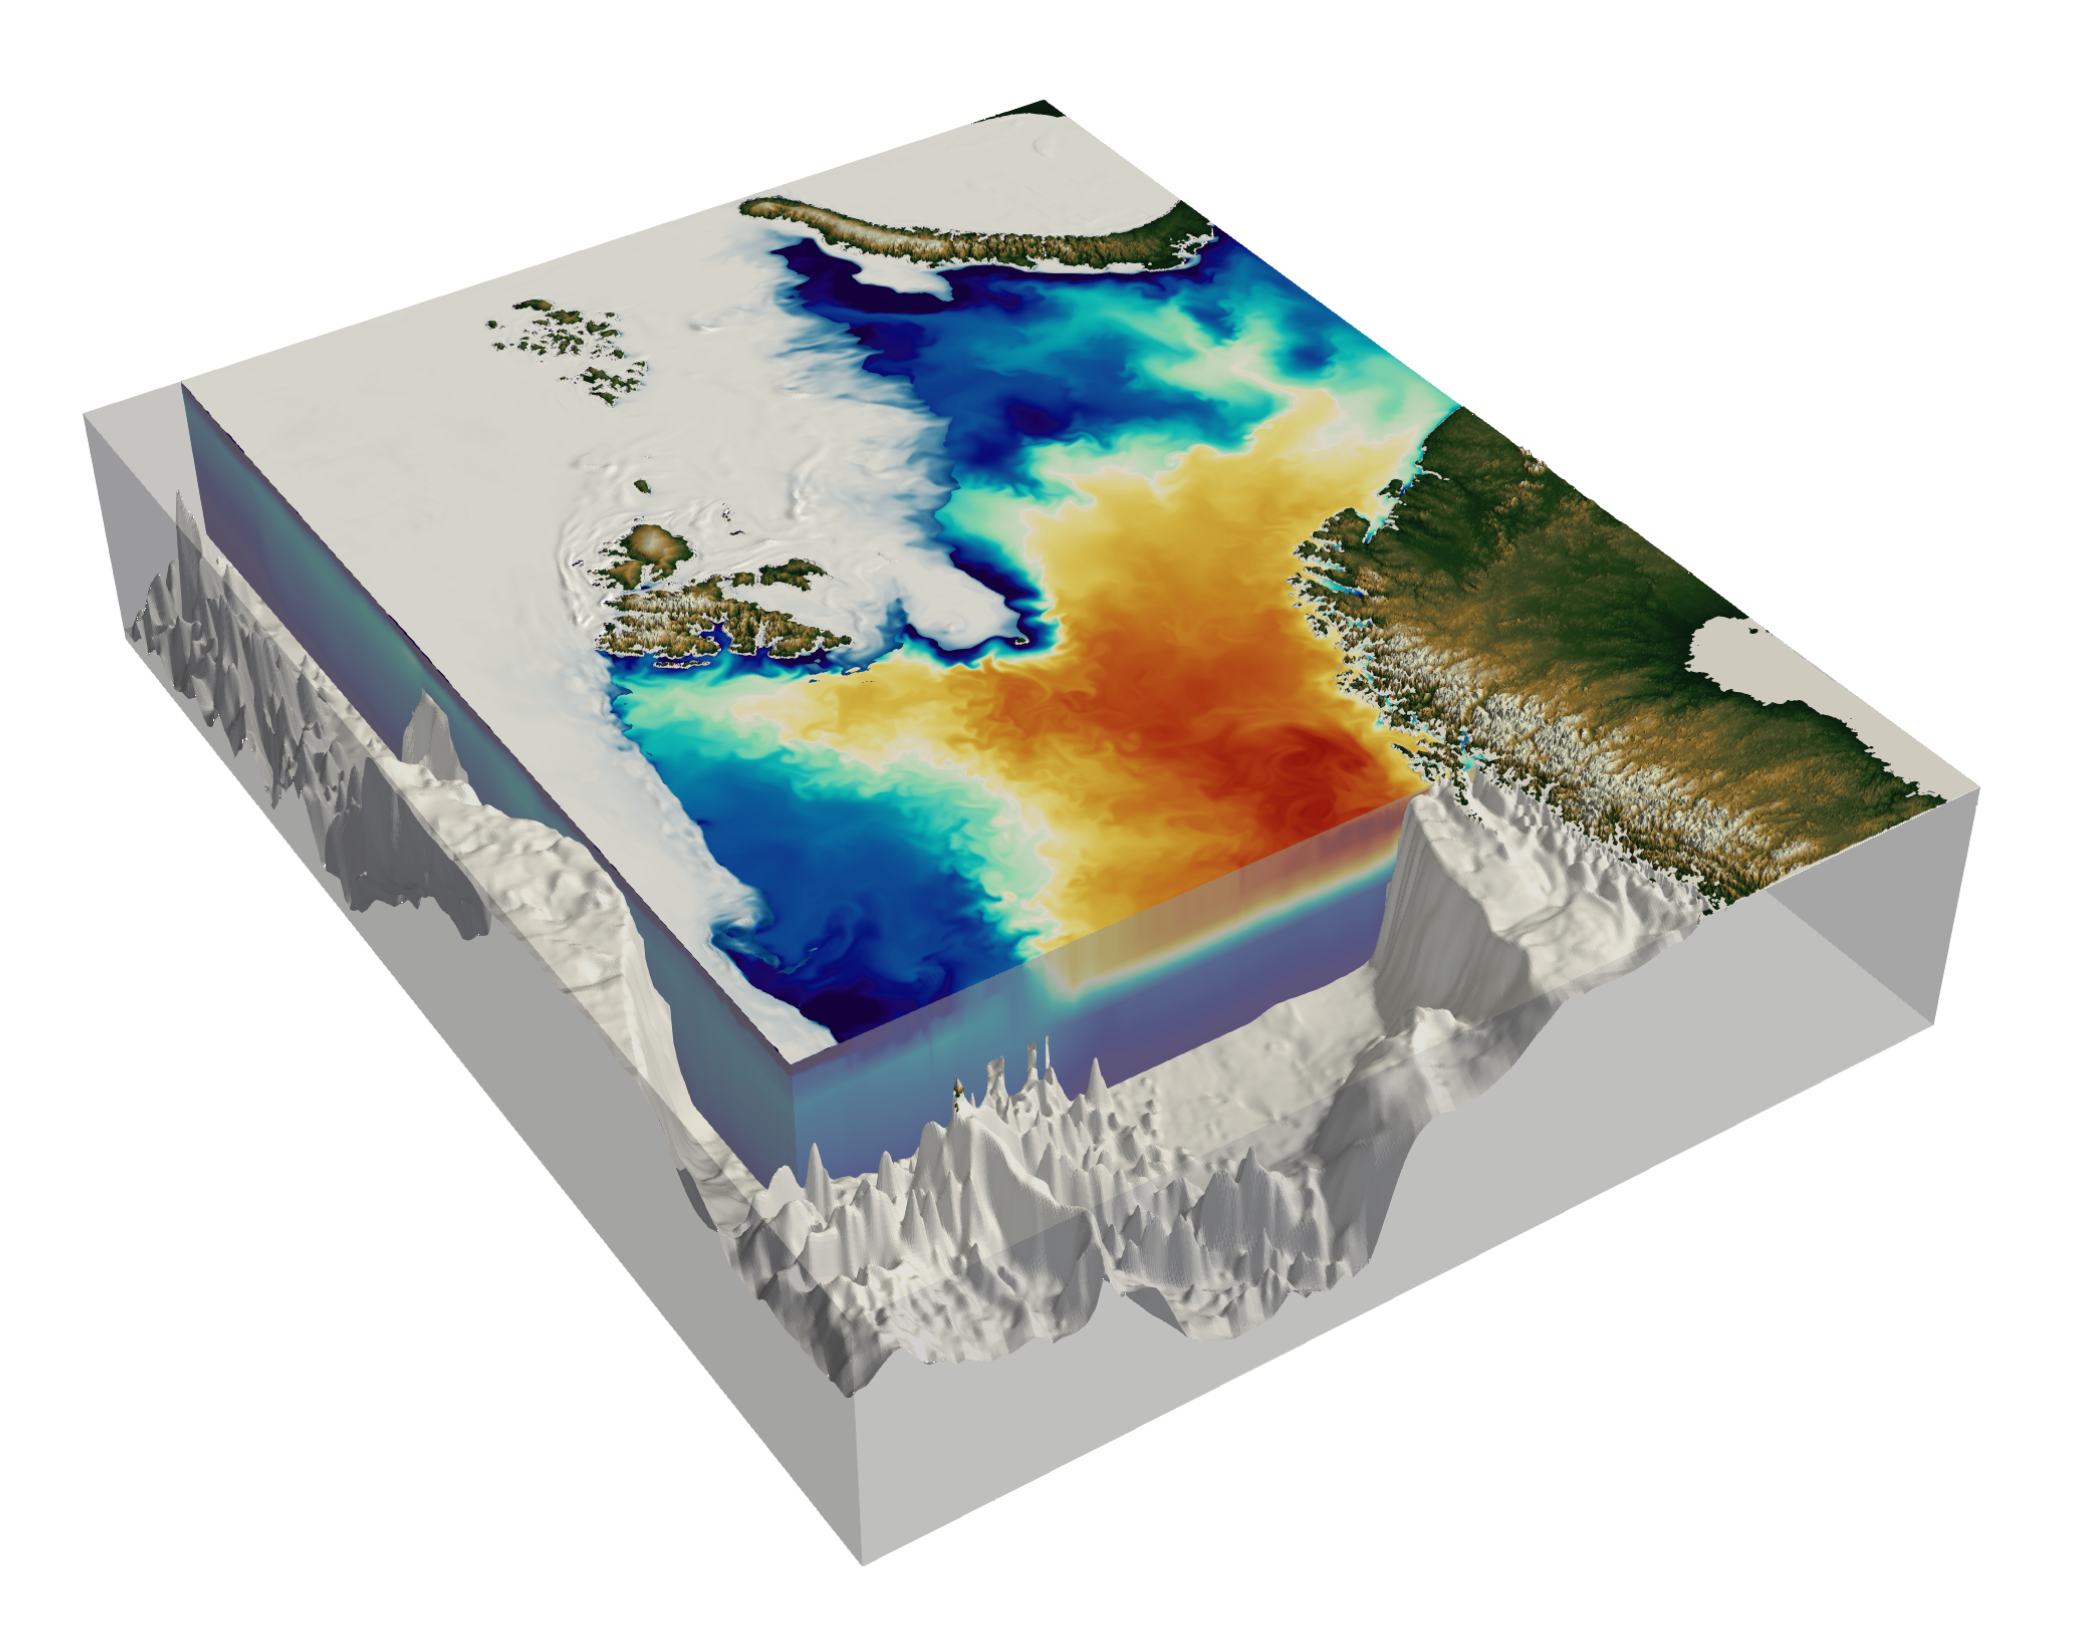
\includegraphics[width=0.75\linewidth]{figures/model_barents_MetNO.png}
    \end{figure}
\end{frame}

%-------------------------------------------------
\begin{frame}{Types of Ocean Models}
\begin{itemize}
\item \textbf{Conceptual models}: diagrams, qualitative ideas, analytical mathematical models
\item \textbf{Statistical and machine-learning models}: based on empirical relationships of data
\item \textbf{Foundation models}: based on deep-learning methods pre-trained on massive ocean datasets
\item \textbf{Dynamical models}: based on physics (focus of this course)
\end{itemize}

\vspace{0.5cm}
\begin{block}{Key idea}
Dynamical models describe how properties change using equations.
\end{block}
\end{frame}

\section{Scales in the ocean}
\begin{frame}{How big are ocean currents?}
\begin{figure}
    \centering
    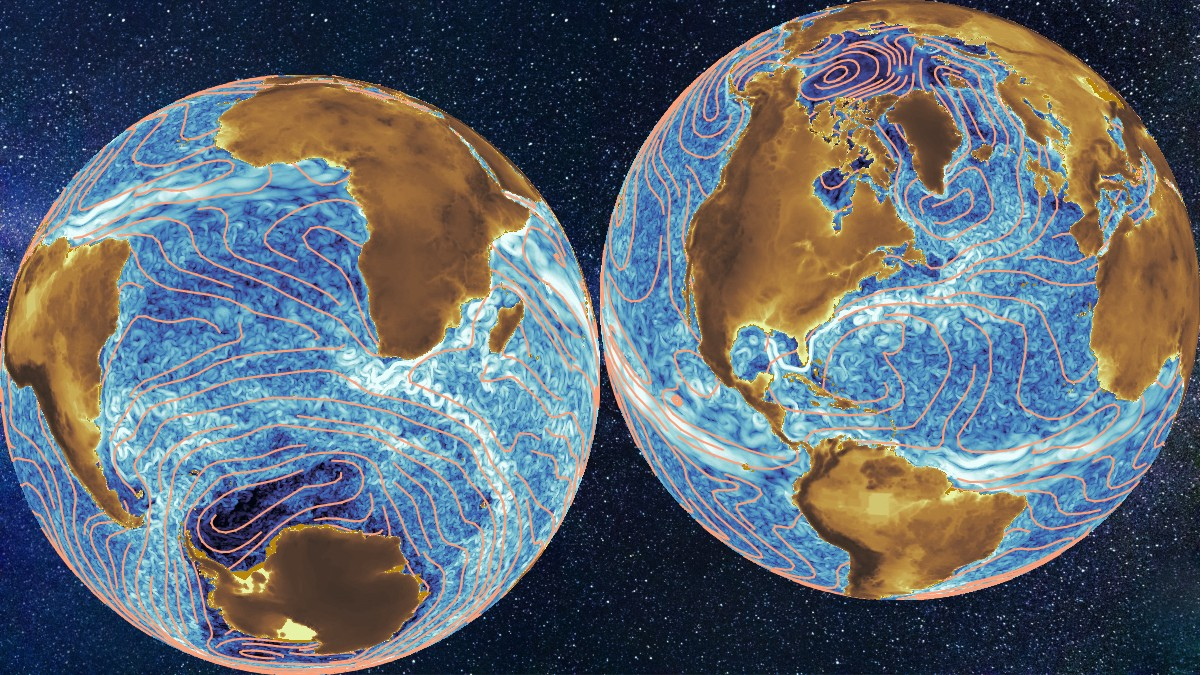
\includegraphics[width=0.5\linewidth]{figures/general_circulation_natcomm.jpg}
    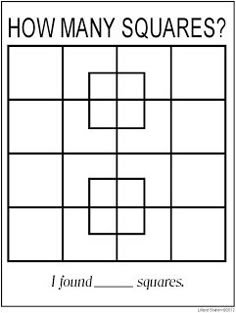
\includegraphics[width=0.2\linewidth]{figures/howmanysquares.jpg}
\end{figure}
With the advent of satellite observations and high-resolution ocean models, it is now possible to observe ocean flow features and analyze how these turbulent oceanic flows of different length scales interact. 

(from \href{https://communities.springernature.com/posts/how-big-are-ocean-currents}{https://communities.springernature.com/posts/how-big-are-ocean-currents})
\end{frame}

%-------------------------------------------------
\begin{frame}{Scales in the physical ocean}

\begin{columns}[t]

\column{7.5cm}

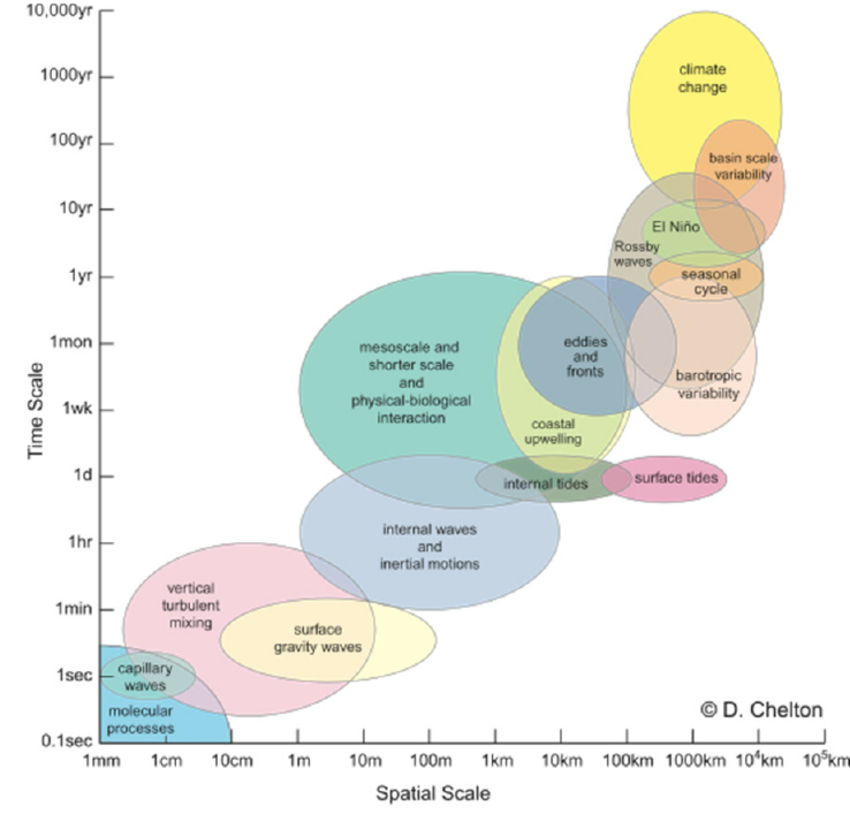
\includegraphics[width=6.3cm]{figures/Time-and-space-scales-of-ocean-variability-courtesy-D-Chelton-Oregon-State-University.png}

\scriptsize{Main time and space scales of ocean variability (D. Chelton, after Dickey (2001)).}

\column{8cm}

\scriptsize{We observe some relationships between the spatial and temporal scales (large phenomena occur at longer time scales, such as El Ni\~no), but processes overlap and span orders of magnitude (the scales are not linear). This figure is associated with the concept of the \textbf{energy cascade}: from the larger to the smaller scales, and to dissipation.
\begin{itemize}
    \item \textbf{El Ni\~no and La Ni\~na}: \href{https://www.youtube.com/watch?v=WPA-KpldDVc}{https://www.youtube.com/watch?v=WPA-KpldDVc}
    \item \textbf{Basin scale circulation + eddies and fronts}: \href{https://www.youtube.com/watch?v=R5-s6O8qyvE}{https://www.youtube.com/watch?v=R5-s6O8qyvE}
    \item \textbf{Internal waves} \href{https://www.youtube.com/watch?v=gYM8cxcyIgI&t=58s}{https://www.youtube.com/watch?v=gYM8cxcyIgI&t=58s}
    \item \textbf{Turbulence at the mesoscale and shorter scales + vertical turbulent mixing}: \href{https://www.youtube.com/watch?v=dNKSrfE2Yv8}{https://www.youtube.com/watch?v=dNKSrfE2Yv8}
\end{itemize}
}

\end{columns}

\end{frame}


\begin{frame}{Physical-biological interactions in marine ecosystems}
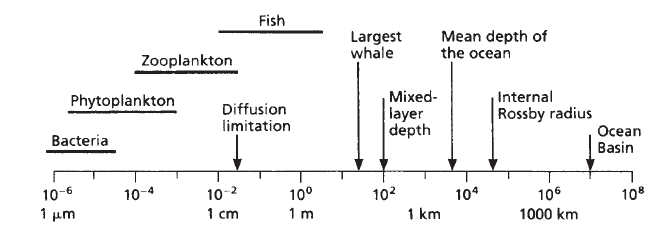
\includegraphics[width=10cm]{figures/scales_mann_lazier.png}
\scriptsize{
\begin{itemize}
\item It is useful to have a feeling for the dimensions of the organisms and phenomena to be discussed (Fig. 1.01, Mann and Lazier, 2006). Ocean basins are typically 10,000 km wide and contain the largest biological communities. Mesoscale processes (i.e. in the order of 100 km in space and in the order of weeks in time) are the main source of variability in water masses and affect the distribution of nutrients and organisms. The average depth of the ocean is 3800 m but the depths of the euphotic layer (~100 m) and the mixed layer (~100 m) are more often critical to open-ocean biological processes. 
\item All marine organisms live at scales that are much smaller than the mesoscale or sub-mesoscale scales and the ocean mixed layer depth. The basis of the food web in the ocean, the plankton ecosystem, is therefore largely affected by microscale processes.
\end{itemize}
}
\end{frame}

%-------------------------------------------------
\section{The Equations of Ocean Models}
%-------------------------------------------------
\begin{frame}{The Ocean as a System of Balance Equations}
The ocean is governed by conservation laws written in terms of \textit{differential equations}:
\begin{itemize}
\item Momentum (movement of water)
\item Mass (continuity)
\item Heat (temperature)
\item Salt (salinity)
\end{itemize}

\vspace{0.5cm}
\begin{block}{Generic form}
\[
\text{Change} = \text{Transport} + \text{Sources} - \text{Sinks}
\]
\end{block}
\end{frame}

%-------------------------------------------------
\begin{frame}{Differential Equations (DE)}
\begin{definition}
\small{Mathematical objects used to describe changes in time and
space. Ordinary DE (ODE) are based on one single independent variable
\[
\frac{dC}{dt}=f\left(C,t,\mathsf{constants}\right);\ \frac{dM}{dx}=f\left(M,x,\mathsf{constants}\right)
\]
$t$ and $x$ are independent variables, the functions
$C(t)$ and $M(x)$ are the solutions of the differential equations. Partial DE work with functions of time and space together (the real ocean): $\frac{\partial \psi}{\partial t},\frac{\partial \psi}{\partial z}$, etc.}

\scriptsize{
\textbf{Types of ODEs}:
\begin{itemize}
\item \textbf{Initial value problem, 0-dimensional (time)}:
this model describes the time evolution of a variable (sea surface
height, phytoplankton population, etc.). The solution is the (continuous)
time series of the variable values, starting from an \emph{initial
condition $C(t=0)$}
\item \textbf{Boundary value problem, 1-dimensional (space)}:
the Lambert-Beer equation is an example of 1-D spatial ODE because
it describes the change with depth of the light distribution. The
solution is a spatial function (in this case, a profile). Spatial ODEs
need a \emph{boundary condition}
\end{itemize}
}
\end{definition}

\end{frame}

%-------------------------------------------------
\begin{frame}{A Mathematical Model for the Ocean}
\small{The three-dimensional Navier-Stokes equation for an incompressible
fluid of constant density in hydrostatic equilibrium on the rotating
earth cannot be resolved analytically. They need numerical representations.}
\begin{align*}
\frac{\partial u}{\partial t}+u\frac{\partial u}{\partial x}+v\frac{\partial u}{\partial y}+w\frac{\partial u}{\partial z}-fv & =-\frac{1}{\rho_{0}}\frac{\partial p}{\partial x}+A_{H}\left(\frac{\partial^{2}u}{\partial x^{2}}+\frac{\partial^{2}u}{\partial y^{2}}\right)+A_{V}\frac{\partial^{2}u}{\partial z^{2}}\\
\frac{\partial v}{\partial t}+u\frac{\partial v}{\partial x}+v\frac{\partial v}{\partial y}+w\frac{\partial v}{\partial z}+fu & =-\frac{1}{\rho_{0}}\frac{\partial p}{\partial y}+A_{H}\left(\frac{\partial^{2}v}{\partial x^{2}}+\frac{\partial^{2}v}{\partial y^{2}}\right)+A_{V}\frac{\partial^{2}v}{\partial z^{2}}\\
\frac{\partial p}{\partial z} & =-\rho_{0}g\\
\frac{\partial u}{\partial x}+\frac{\partial v}{\partial y}+\frac{\partial w}{\partial z} & =0\\
\frac{\partial T}{\partial t}+u\frac{\partial T}{\partial x}+v\frac{\partial T}{\partial y}+w\frac{\partial T}{\partial z} & =\kappa_{H}\left(\frac{\partial^{2} T}{\partial x^{2}}+\frac{\partial^{2} T}{\partial y^{2}}\right)+\kappa_{V}\frac{\partial^{2} T}{\partial z^{2}}\\
\frac{\partial S}{\partial t}+u\frac{\partial S}{\partial x}+v\frac{\partial S}{\partial y}+w\frac{\partial S}{\partial z} & =\kappa_{H}\left(\frac{\partial^{2}S}{\partial x^{2}}+\frac{\partial^{2}S}{\partial y^{2}}\right)+\kappa_{V}\frac{\partial^{2}S}{\partial z^{2}}
\end{align*}

\end{frame}


%-------------------------------------------------
\begin{frame}{Example: Temperature Equation (1-dimensional)}
\[
\frac{\partial T}{\partial t} + u \frac{\partial T}{\partial x} = \kappa \frac{\partial^2 T}{\partial x^2}
\]

\begin{itemize}
\item Left term: change in time
\item Middle term: transport by currents (advection)
\item Right term: mixing (diffusion)
\end{itemize}

\begin{block}{Interpretation}
Temperature changes because water moves and mixes. Note that we have neglected other thermal drivers like solar heating. They are also included in the equations.
\end{block}
\end{frame}

%-------------------------------------------------
\section{From Reality to Equations to Numerical Solutions: \\the Discrete Ocean}
%-------------------------------------------------
\begin{frame}{Numerical Ocean Models are not reality (but are very useful)}
\begin{block}{Some Challenges:}
\end{block}
\begin{itemize}
\item {The numerical equations driving the model are \textbf{approximations}
of the mathematical equations that describe fluid flow.}
\item {Models do not contain information about the flow features between grid points (discrete information)}.
\item Not every process in the ocean is understood and represented by a mathematical formulation.
\item Processes that are smaller than the grid cell, or that are not fully resolve must be \textit{parameterized}.
\item Numerical discretization biases due to the approximated solution or the choice of the grid
\end{itemize}
\end{frame}

%-------------------------------------------------
\begin{frame}{From the Continuous Ocean to Numerical Models}
\begin{columns}
\column{6cm}
Reality:
\begin{itemize}
\item Continuous ocean
\item Infinite detail
\end{itemize}

Model:
\begin{itemize}
\item Discrete grid (cells and nodes)
\item Finite number of points
\end{itemize}

\column{8cm}
\begin{figure}
    \centering
    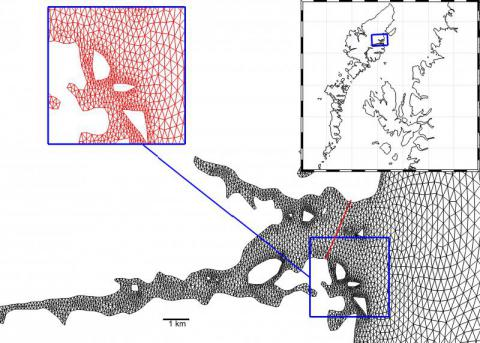
\includegraphics[width=0.75\linewidth]{figures/grid_type-ssm_eclh_unstructured_grid.jpg}
\end{figure}
\end{columns}
\end{frame}


%-------------------------------------------------
\begin{frame}{Types of Numerical Ocean Models}
\small{
\begin{table}[]
\centering
\begin{tabular}{lccc}
\hline
\textbf{Feature} & \textbf{Free-Run Models} & \textbf{Ocean Reanalyses} & \textbf{Climate Models}\\
\hline
Data Assimilation & No & Yes & No \\
Realism vs Observations & Medium & Higher & Lower \\
Drift Over Time & Possible & Reduced & Unconstrained \\
Primary Use & Process understanding & State estimation & Future projections \\
\hline
\end{tabular}
\end{table}
\vspace{0.5cm}
\textbf{Key Idea:}
\begin{itemize}
\item Free-run models explore \textit{what could happen} 
\item Reanalyses aim at reconstructing \textit{what actually happened}
\item Climate models, which include many other components of the Earth System and not only the ocean, \textit{explore scenarios of climate change}
\end{itemize}
}
\end{frame}

%-------------------------------------------------
\begin{frame}{Free-Run Ocean Models}
\small{
\begin{columns}
\column{0.5\linewidth}
\textbf{Core Features:}
\begin{itemize}
\item Numerical simulations driven by atmospheric forcing and other boundary conditions
\item Can be 1-D, 2-D or 3-D, depending on the questions
\item No assimilation of observational data
\end{itemize}
\textbf{Characteristics:}
\begin{itemize}
\item Governed by model physics, initial and boundary conditions
\item Internal variability is dynamically consistent
\item Errors (including numerical errors) can grow generating model drift
\end{itemize}
\column{0.5\linewidth}
\textbf{Strengths:}
\begin{itemize}
\item Ideal for process studies and sensitivity experiments
\item Physically self-consistent system
\end{itemize}
\textbf{Limitations:}
\begin{itemize}
\item May diverge from the observed ocean state
\item Depends strongly on knowledge of physical processes and forcing/boundary data accuracy
\end{itemize}
\end{columns}
}
\end{frame}

%-------------------------------------------------
\begin{frame}{Ocean Reanalyses: \href{https://www.youtube.com/watch?v=FAGobvUGl24}{https://www.youtube.com/watch?v=FAGobvUGl24}}
\small{
\begin{columns}
\column{0.5\linewidth}
\textbf{Core Features:}
\begin{itemize}
\item Model simulations constrained by observations
\item Assimilate data (Argo, satellites, moorings, etc.)
\end{itemize}
\textbf{Characteristics:}
\begin{itemize}
\item Combines model dynamics with real-world measurements
\item Regular corrections toward observed state
\item Produces consistent, observation-based datasets
\end{itemize}
\column{0.5\linewidth}
\textbf{Strengths:}
\begin{itemize}
\item Closest estimate of the real ocean state
\item Essential for validation and climate monitoring
\end{itemize}
\textbf{Limitations:}
\begin{itemize}
\item Same as the previous ones. One cannot correct a physically inaccurate model with data
\item Sensitive to data coverage and assimilation methods
\item Can include temporal inconsistencies or nonphysical responses
\end{itemize}

\end{columns}
}
\end{frame}

%-------------------------------------------------
\begin{frame}{Ocean Models in Climate Simulations: \href{https://www.youtube.com/watch?v=fzEHTxKJOjI}{https://www.youtube.com/watch?v=fzEHTxKJOjI}}
\small{
\begin{columns}
\column{0.5\linewidth}
\textbf{Core Features:}
\begin{itemize}
\item Coupled to atmosphere, sea ice, and land components
\item Solve primitive equations on a global grid
\item Include parameterizations for unresolved processes
\end{itemize}

\textbf{Characteristics:}
\begin{itemize}
\item Stratification and thermohaline circulation
\item Air--sea flux exchange (heat, momentum, freshwater)
\item Mesoscale eddies (resolved or parameterized)
\end{itemize}
\column{0.5\linewidth}
\textbf{Strengths:}
\begin{itemize}
\item Project future ocean and climate states
\item Long integrations (decades to centuries)
\item Designed for stability and energy conservation
\end{itemize}

\textbf{Limitations:}
\begin{itemize}
\item Computational costs
\item Coarse to eddy-permitting resolution (improving)
\item Many unconstrained sub-grid scale parameterizations
\end{itemize}
\end{columns}
}
\end{frame}


%-------------------------------------------------
\begin{frame}{The Numerical Grid}
\begin{center}
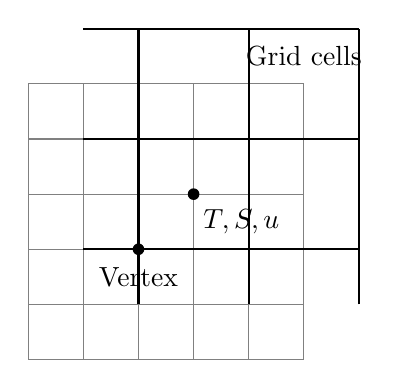
\begin{tikzpicture}[scale=0.7]
\draw[step=1cm,gray,thin] (0,0) grid (5,5);
\draw[step=2cm,black,thick] (1,1) grid (6,6);
\fill[black] (3,3) circle (3pt);
\fill[black] (2,2) circle (3pt);
\node at (2,1.5) {Vertex};
\node at (5,5.5) {Grid cells};
\node[right] at (3,2.5) {$T,S,u$};
\end{tikzpicture}
\end{center}

\begin{itemize}
\item The ocean is divided into grid cells, with vertices and nodes
\item Each cell stores variables (T, S, velocity)
\item Interactions occur between neighbouring cells
\end{itemize}
\end{frame}

%-------------------------------------------------
\begin{frame}{Key Concept: Resolution}
\begin{columns}
\column{6cm}
\begin{itemize}
\item Grid spacing controls what we can resolve
\item Fine grid means more detail (eddies, fronts)
\item Coarse grid can resolve the large-scale circulation only
\end{itemize}
\begin{block}{Important}
Processes smaller than the grid must be approximated ("parameterized")
\end{block}
\column{8cm}
\begin{figure}
    \centering
    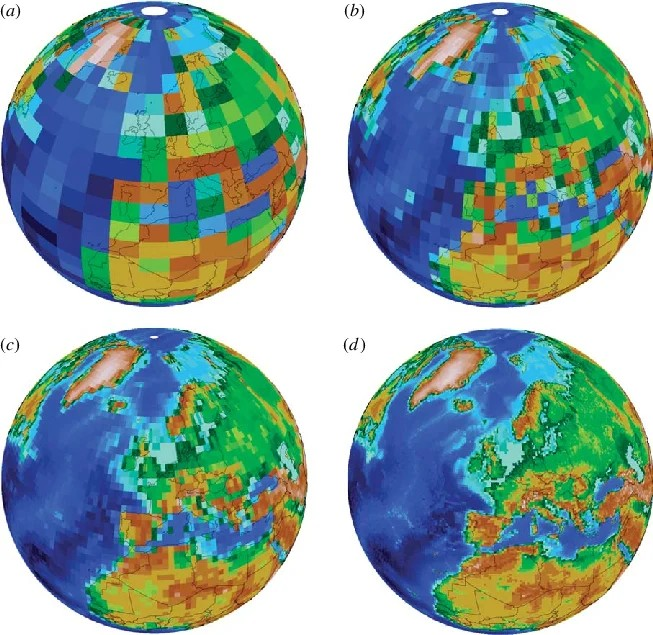
\includegraphics[width=0.7\linewidth]{figures/Horizontal-resolution-comparison.jpg}
\end{figure}
\end{columns}
\end{frame}

%-------------------------------------------------
\begin{frame}{The Monash Simple Climate Model: \url{https://www.monash.edu/mcccrh/climate-communicators/completed/MSCM}}
The Monash University Interactive Simple Climate Model (MSCM) is a web-based interface that allows users to explore the physical simulation of the climate system with a real global climate model. Despite its simplicity and coarse resolution, the model simulates the climate response to external forcings, such as the doubling of carbon dioxide concentrations, very realistically.
\begin{figure}
        \centering
        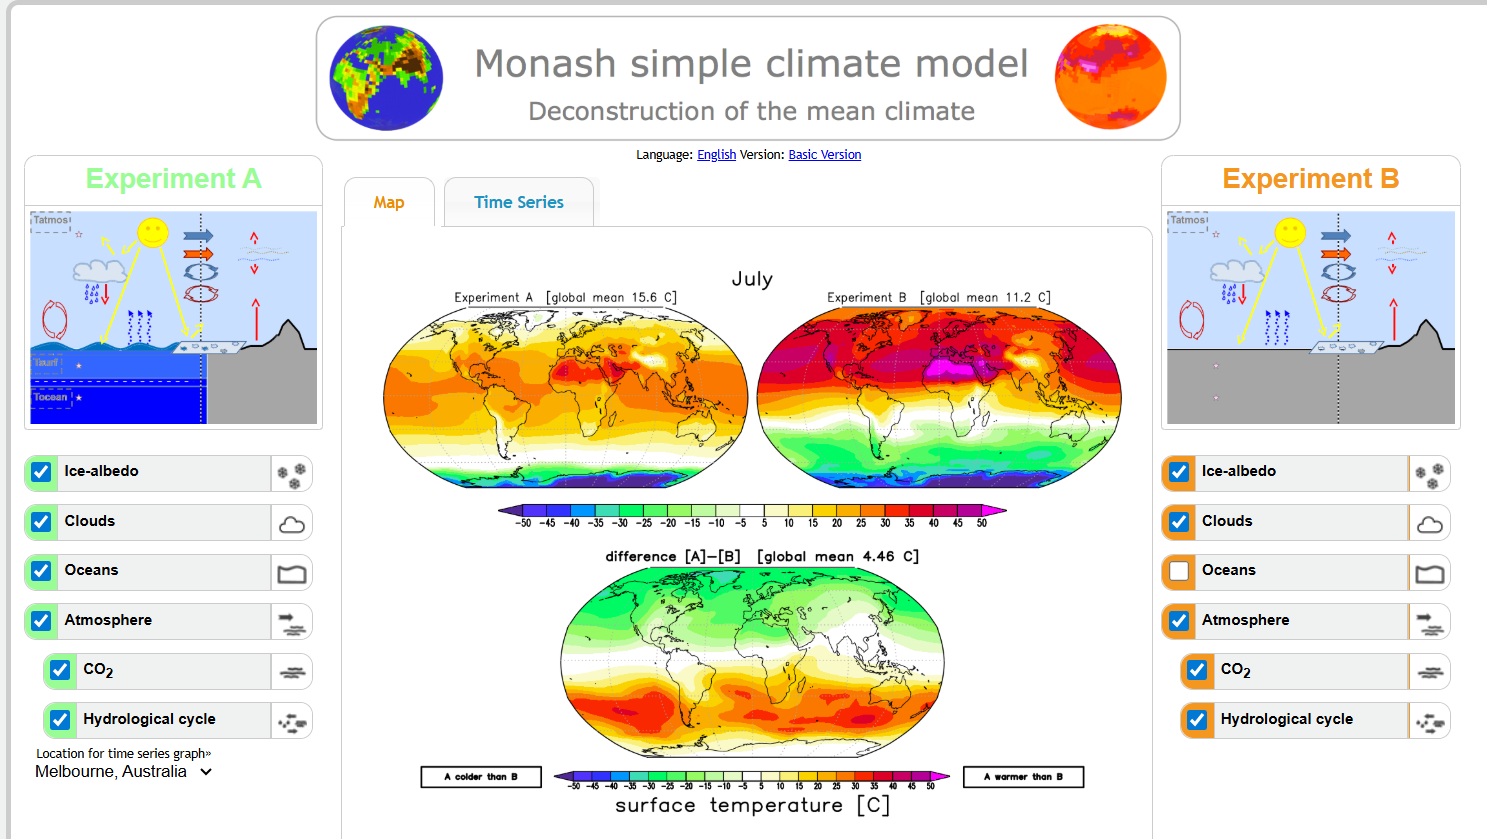
\includegraphics[width=0.5\linewidth]{figures/monash_simple_CM.png}
    \end{figure}    
\end{frame}

\begin{frame}{Exercise US2.4-oce1: the Role of the Ocean in the Climate System}
    \begin{itemize}
        \item Use the Basic Version of the model to deconstruct the mean climate of the Earth
        \item Run two simulations: 1) with and without the effect of the ocean and 2) with and without the sea-ice albedo feedback (with the ocean turned on). Familiarize yourself with the concept of sea ice - albedo feedback
        \item In maximum 2 pages, including figures, briefly explain the differences in surface maps, and the implications on the seasonal cycle of surface temperature in Melbourne, Australia. 
        \item Submit the PDF on Amathuba
    \end{itemize}
\end{frame}

%-------------------------------------------------
\section{Model Classification}
%-------------------------------------------------
\begin{frame}{Classification of Ocean Models}
\begin{block}{Definition}
Models are classified according to the \textbf{domain extent}, the \textbf{components}, and the approaches used to represent the \textbf{horizontal grid} and the \textbf{vertical coordinate system}.
\end{block}
\begin{figure}
    \centering
    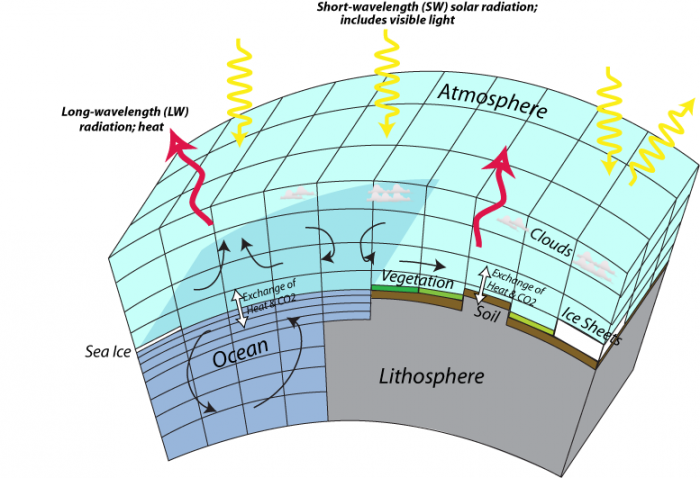
\includegraphics[width=0.65\linewidth]{figures/GCM_grid_components.png}
\end{figure}
    
\end{frame}

%-------------------------------------------------
\frame{
\frametitle{Main Criteria for Classification}
\begin{itemize}
\item {Geography (domains)} \vspace{0.2in}
 
\item {Processes (components)} \vspace{0.2in}
  
\item {Discretization of the horizontal and vertical grids (Grid cell size and vertical structure of the water column)}
\end{itemize}
}

%-------------------------------------------------
\begin{frame}{Geographic classification: domain size}
\begin{columns}
\column{0.4\linewidth}
\begin{itemize}
\item {Global scale (the entire ocean)} 
\item {Basin scale or regional (the Atlantic Ocean)} 
\item {Local or coastal scale (the Southern Benguela)} 
\end{itemize}
\column{0.6\linewidth}
\begin{figure}
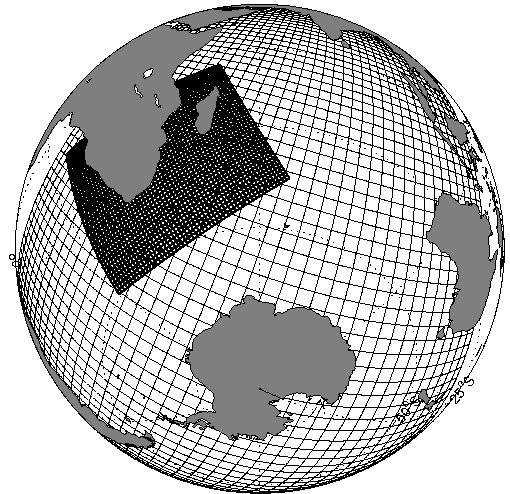
\includegraphics[width=1\linewidth]{figures/globalgrid} 
\end{figure}
\end{columns}    
\end{frame}

%-------------------------------------------------
\begin{frame}{Nested grids}
\begin{block}{Parent and children}
Regional models are often built with a combination of nested grids,
from a parent grid at coarser resolution to children at higher resolutions.
All regional models need boundary conditions. The boundary can be
passive (one-way coupling from the parent to the child) or active (two-way coupling). From Fearon et al. (2023). 
\end{block}
\begin{figure}
    \centering
    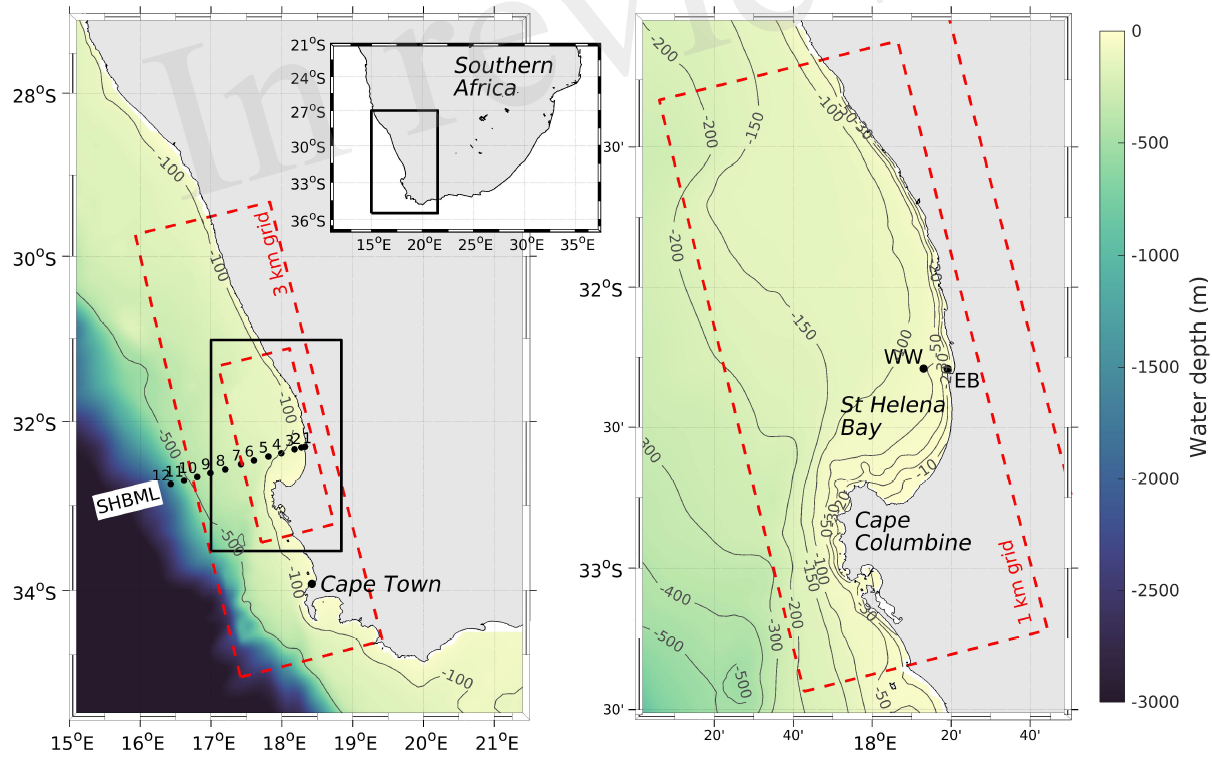
\includegraphics[scale=0.3]{figures/Benguela-nesting}
\end{figure}
\end{frame}

%-------------------------------------------------
\begin{frame}{Vertical grid discretization}
There are several choices for the vertical coordinate system. All choices allow to increase detail near the surface where most of the energy exchange occurs. \textcolor{red}{However, they all have strengths and limitations}. The 4-most used coordinates are:
\begin{itemize}
\item {\textcolor{blue}{Fixed-Level, Geopotential or Z-Coordinate model}} 
\item {\textcolor{blue}{Isopycnal-coordinate model}} 
\item {\textcolor{blue}{Sigma or Stretched-coordinate model}} 
\item {\textcolor{blue}{Hybrid-coordinate model}} 
\end{itemize}
\end{frame}

%-------------------------------------------------
\begin{frame}{Vertical coordinates}
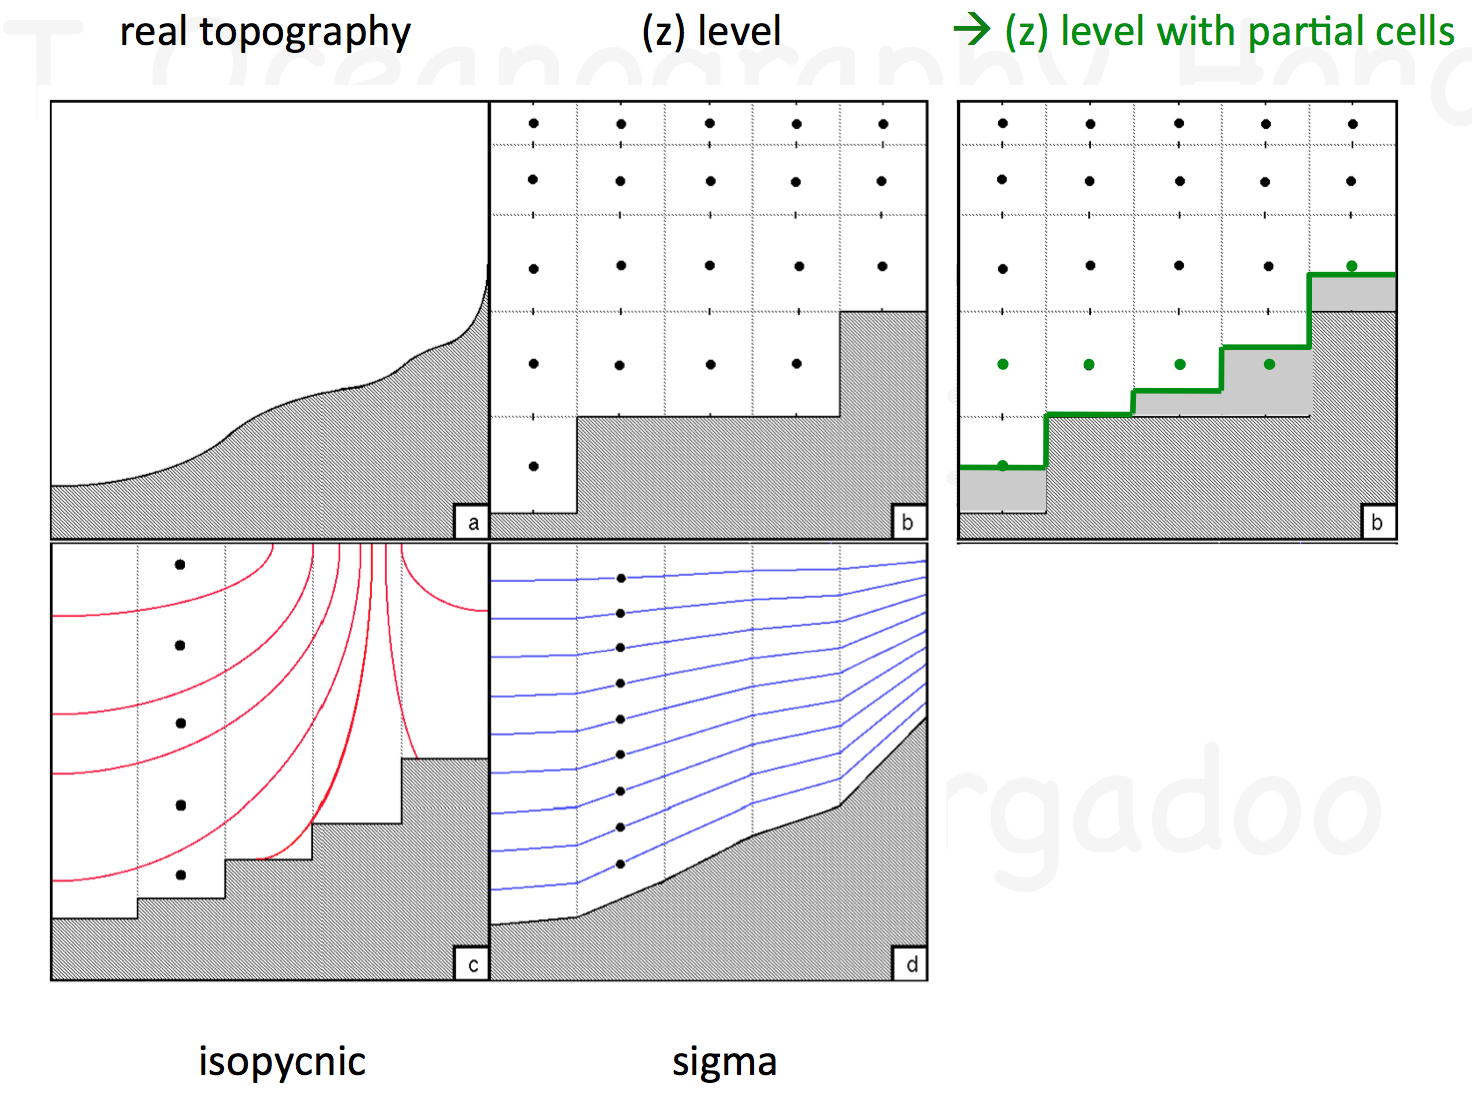
\includegraphics[width=0.6\paperwidth]{figures/vertical-coordinates}
Courtesy of J. Doorgadoo
\end{frame}

%-------------------------------------------------
\begin{frame}{Z-Coordinate}
\begin{columns}
    \column{0.4\linewidth}
    \begin{figure}
     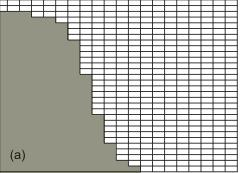
\includegraphics[width=1\linewidth]{figures/z-coord} 
    \end{figure}
    \column{0.6\linewidth}
\begin{itemize}
\item {Consists of a series of regular surface depths. It is easy to set-up and is computationally efficient.}
\item The topography resolution is increased by decreasing the spacing between the levels.
\item There is no easy-way to increase vertical resolution without adding cells to the entire model domain.
\item It has a poor representation of the continental slope, but it can be alleviated through partial cells. 
\end{itemize}    
\end{columns}
\end{frame}

%-------------------------------------------------
\begin{frame}{Isopycnal coordinates: \href{https://www.youtube.com/watch?v=8VMSF28J9H4}{https://www.youtube.com/watch?v=8VMSF28J9H4}}
\begin{columns}
\column{0.3\linewidth}
\begin{figure}
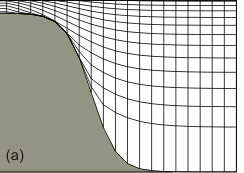
\includegraphics[width=1\linewidth]{figures/isopyc-coord} 
\end{figure}
\column{0.8\linewidth}
\begin{itemize}
\item The ocean is described by a set of \textbf{non-mixing layers} whose interface depths in every grid cell adjust in time driven by the physics.
\item Equations of motion are calculated in each isopycnal layer, that are interfaces of equal density. The main state variables are the layer-averaged velocity and layer thickness. 
\item Mixing of water properties across the layers can be neglected because the layers are moved up, down, or squeezed, depending on changes in heat and salt. Perfect for following water masses.
\item The main disadvantage is that these models perform poorly in shallow waters where there is a variable mixed layer depth that can extend through the whole depth. Isopycnals do not naturally follow the seafloor.
\end{itemize}
\end{columns}
\end{frame}

%-------------------------------------------------
\begin{frame}{Sigma-Coordinate or terrain-following}
\begin{columns}
\column{0.4\linewidth}
\begin{figure}
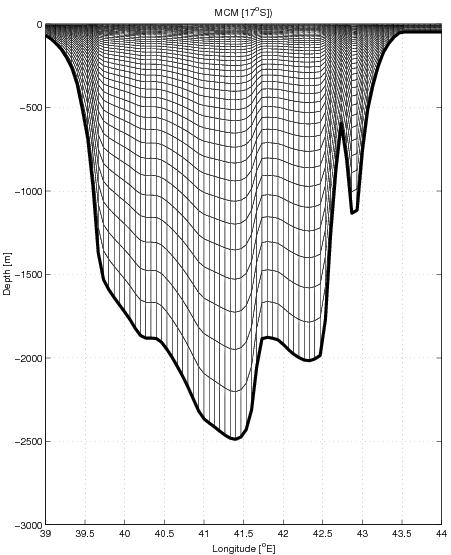
\includegraphics[width=1\linewidth]{figures/sig-coord} 
\end{figure}
\column{0.6\linewidth}
\begin{itemize}
\item Assume coordinate surfaces which are fixed in time, but follow
the underlying topography. 
\item Resolve the lateral boundaries and complex bathymetry. Fairly horizontal near the ocean surface, and follow the bathymetry near the seafloor.
\item Allow for a better representation of the flow over the bathymetry. 
\item Can cause instabilities where the topography is very steep because levels can get very close to each other. The number of levels is the same everywhere in the domain.
\end{itemize}
\end{columns}
\end{frame}


%-------------------------------------------------
\begin{frame}{Hybrid coordinates}
\begin{columns}
\column{0.4\linewidth}
\begin{figure}
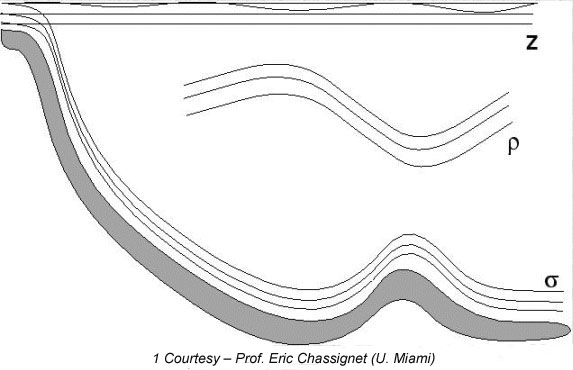
\includegraphics[width=1\linewidth]{figures/hyb-coord} 
\end{figure}
\column{0.6\linewidth}
\begin{itemize}
\item Optimise model performance by combining the most adequate coordinate systems in different regions based on the dominant process.
\item Good representation of the vertical structure of the ocean throughout the water column.
\item Allow the vertical coordinates to evolve in time and space as the depth of the mixed layer changes.
\item High computational cost and complex data visualization procedures. 
\end{itemize}
\end{columns}
\end{frame}

%-------------------------------------------------
\frame{
\frametitle{Horizontal grids}
There are two main types of horizontal grids, each one with several sub-categories or nuances.
\begin{itemize}
\item {\textcolor{blue}{Structured grids} (finite volumes; regular or irregular/curvilinear)} 
\item {\textcolor{blue}{Unstructured grids} (finite elements, best way
to approximate a coastline)} 
\end{itemize}
\begin{figure}
    \centering
    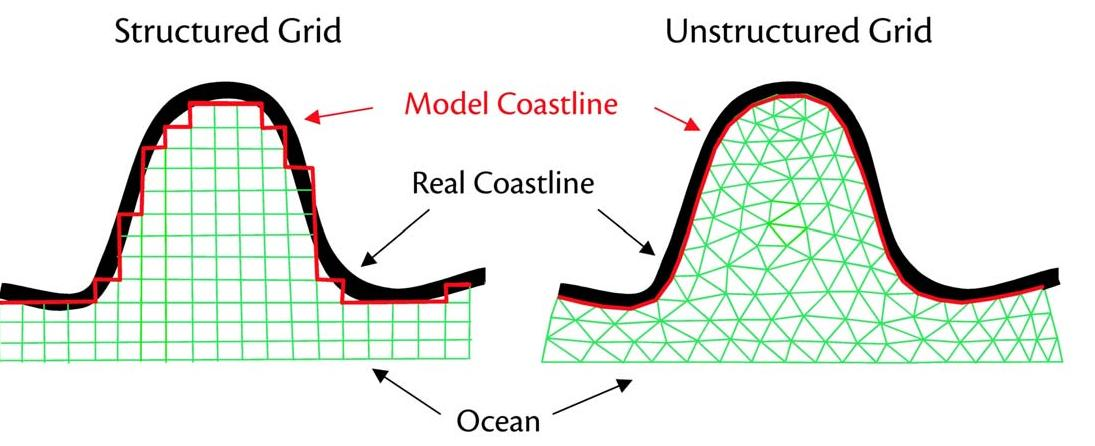
\includegraphics[scale=0.3]{figures/regular_irregular_grids} 
\end{figure}
}

%-------------------------------------------------
\frame{
\frametitle{Horizontal structured grids}
\begin{block}{Structured Grids (Rectangular, Curvilinear and
Spherical)}
Consist of a series of spaced orthogonal lines. 
\end{block}
\begin{itemize}
\item Neighbouring cells can be identified in a structured way
\item Are computationally efficient. 
\item Use straightforward algorithms intuitively derived from the discretized equations.
\item Because the surface of the earth is a sphere, we cannot truly apply a uniform spacing across the grid and keep the lines straight. It also generates problems at the North pole, which is in the Arctic Ocean.
\end{itemize}
} 

%-------------------------------------------------
\begin{frame}{Grids on the Earth surface}
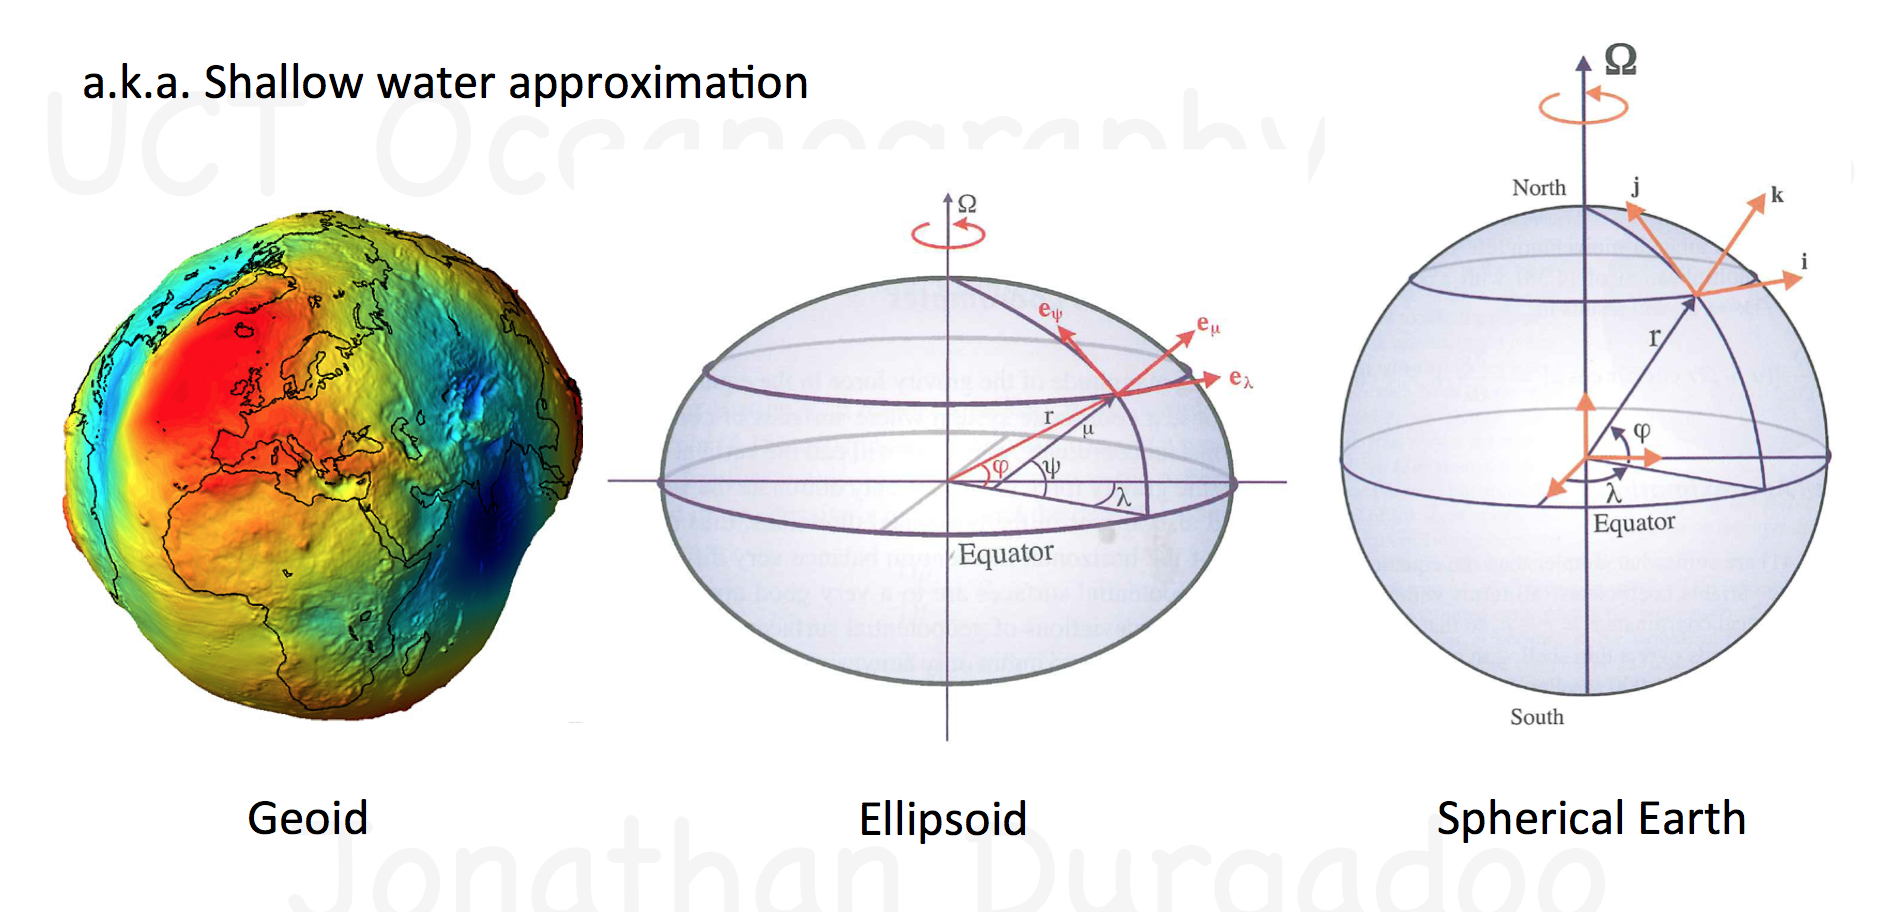
\includegraphics[width=0.8\paperwidth]{figures/spherical}
\end{frame}

%-------------------------------------------------
\begin{frame}{Spherical Earth grids: the tri-polar grid}
\begin{columns}
\column{0.6\linewidth}
\begin{figure}
    \centering
    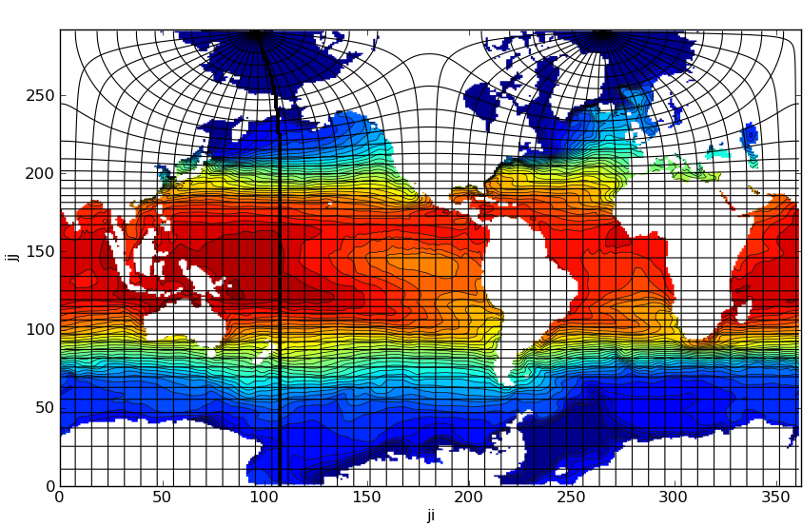
\includegraphics[width=1\linewidth]{figures/grid_type-orca2.jpg}
\end{figure}
\column{0.4\linewidth}
\begin{figure}
    \centering
    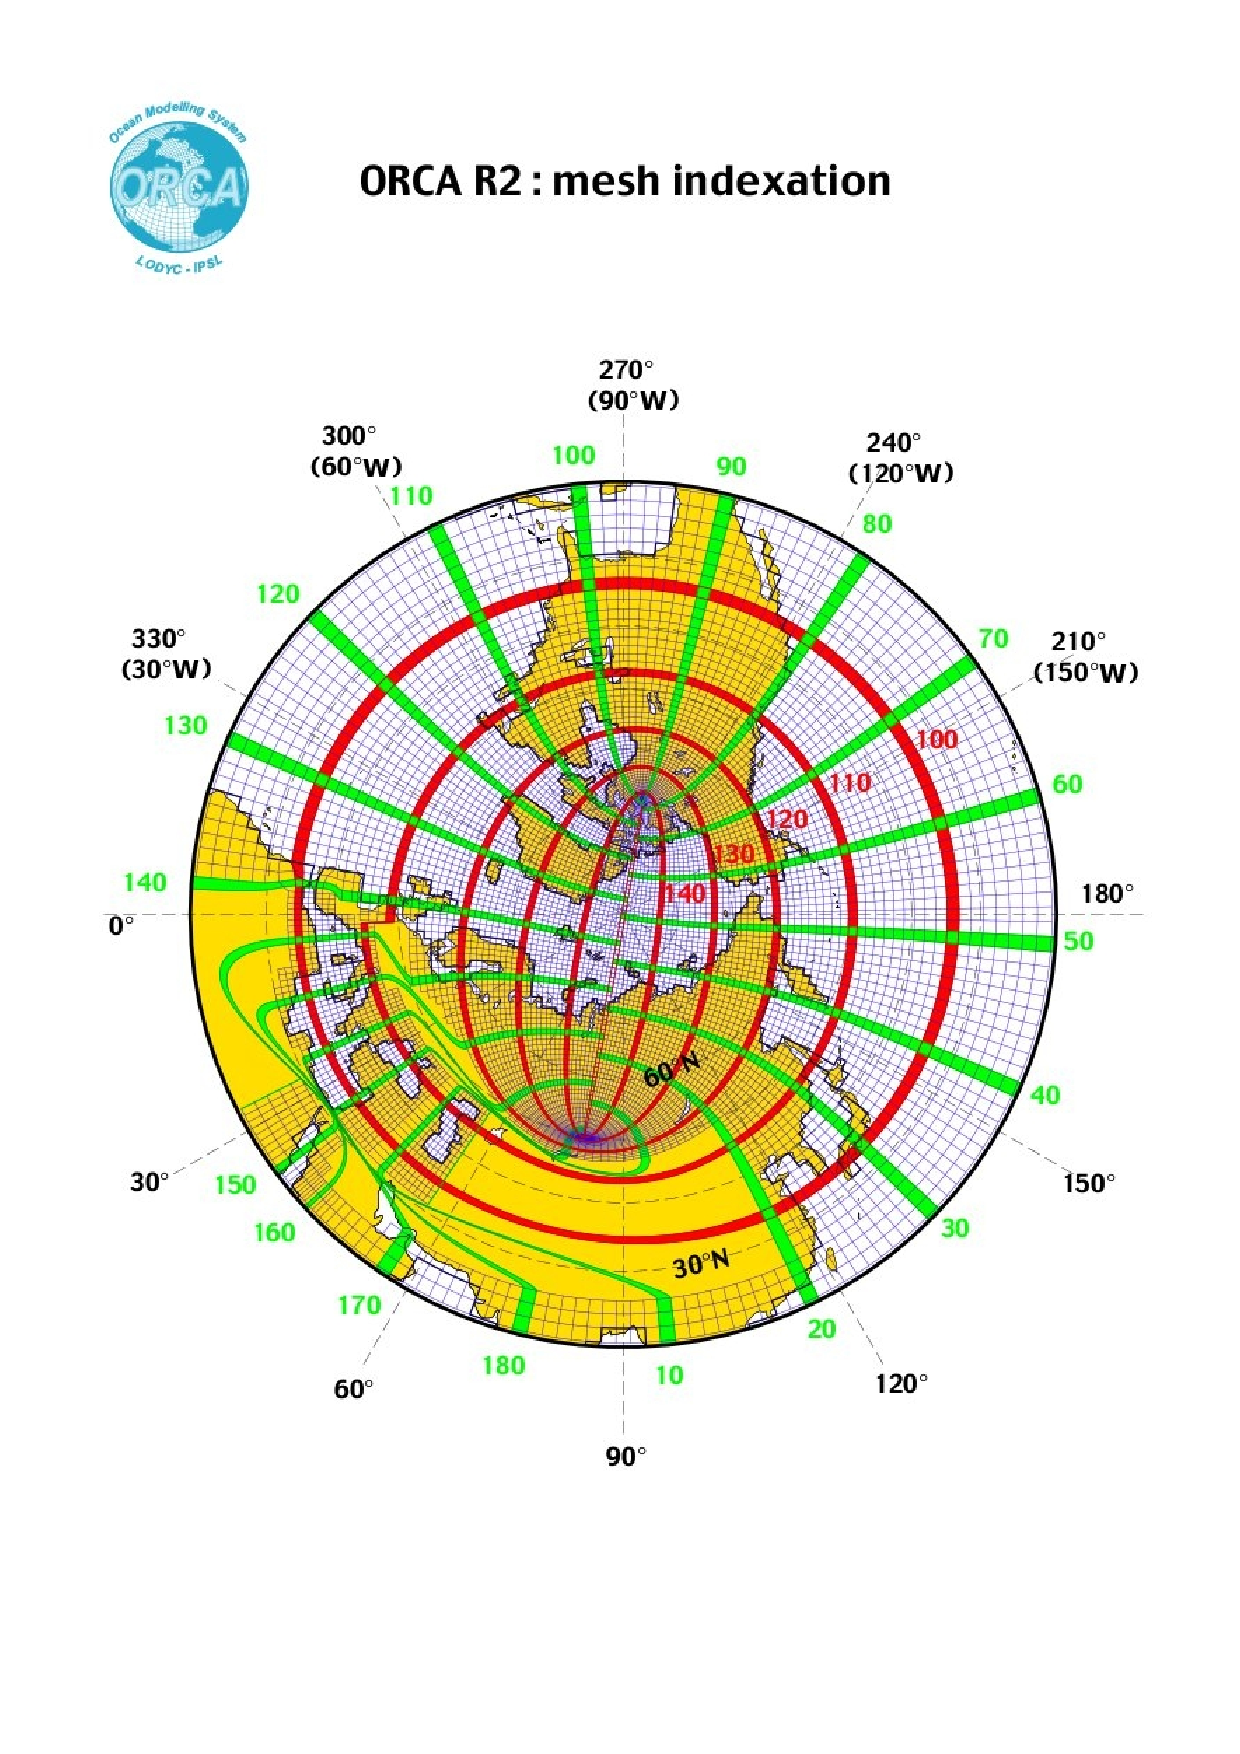
\includegraphics[width=1\linewidth]{figures/ORCA2_north_pole_mesh}
\end{figure}
\end{columns}
\end{frame}

%-------------------------------------------------
\begin{frame}{Unstructured grids (finite elements and finite volumes)}
\begin{block}{Also called triangular grids, they consist of a series of triangles or other more versatile polygons}
\end{block}
\begin{itemize}
\item {\textcolor{blue}{Developed specially for the regional coastal ocean
and estuaries.}} 
\item {\textcolor{blue}{Allows to increase the resolution near the coast
where small-scale processes are important, while keeping coarser resolutions
where not required}}
\item {\textcolor{blue}{Can be more difficult to set-up and need specialized
algorithms}} 
\item {\textcolor{blue}{Computationally expensive}} 
\end{itemize}
\end{frame}

%-------------------------------------------------
\begin{frame}{Unstructured grid models (global ocean example)}

\begin{figure}
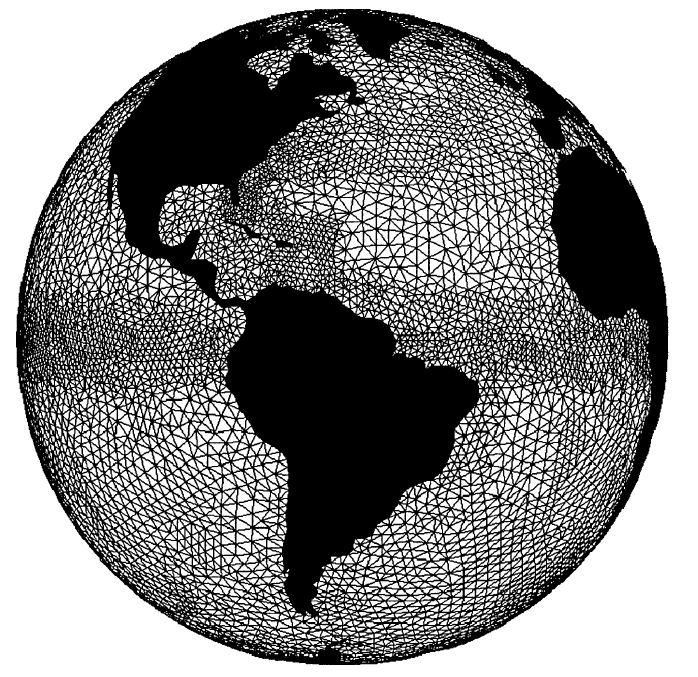
\includegraphics[scale=0.3]{figures/unstructured_grid}
\end{figure}

\end{frame}

%-----------------------------
\begin{frame}{Overview of the Major Ocean Numerical Models}

\textbf{General circulation / primitive equation models}
\begin{itemize}
    \item \textbf{MOM (NOAA/GFDL)} 
    {\footnotesize \url{https://mom-ocean.github.io}}
    
    \item \textbf{NEMO} 
    {\footnotesize \url{https://www.nemo-ocean.eu}}
    
    \item \textbf{MITgcm} 
    {\footnotesize \url{http://mitgcm.org}}
\end{itemize}

\textbf{Terrain-following / coastal models}
\begin{itemize}
    \item \textbf{ROMS and CROCO} 
    {\footnotesize \url{https://www.myroms.org} \url{https://www.croco-ocean.org}}
    
    \item \textbf{FVCOM} 
    {\footnotesize \url{https://fvcom.smast.umassd.edu}}
\end{itemize}

\textbf{Key features}
\begin{itemize}
    \item Structured vs unstructured grids
    \item Hydrostatic vs non-hydrostatic
\end{itemize}

\end{frame}

%-----------------------------
\begin{frame}{Advanced and Specialized Models}

\textbf{Unstructured / adaptive mesh models}
\begin{itemize}
    \item \textbf{FESOM} 
    {\footnotesize \url{https://fesom.de}}
    
    \item \textbf{MPAS-Ocean} 
    {\footnotesize \url{https://mpas-dev.github.io}}

    \item \textbf{HYCOM} 
    {\footnotesize \url{https://www.hycom.org}}
\end{itemize}

\textbf{Key features}
\begin{itemize}
    \item Grid: structured vs unstructured
    \item Vertical coordinates: $z$, $\sigma$, isopycnal, hybrid
    \item Applications: climate, coastal, multi-scale
\end{itemize}

\centering
\small \textit{All models solve the same physics, but parameterizations and numerical schemes are different. Model choice depends on scale, geometry, and questions}

\end{frame}

%-------------------------------------------------
\section{\textit{Running} the Model \\ \url{https://github.com/mvichi/SAMOS-ocean-modelling-UCT}}
%-------------------------------------------------
\begin{frame}{How Does the Model Work?}
Models are sophisticated software, developed by large teams. Individual researchers do not create their own models: either work with idealised models, or very often adapt existing model engines to their problem.
The models are run, which means they are executed given a choice of grid, bathymetry, and atmospheric/lateral boundary conditions. At each time step:
\small{
\begin{enumerate}
\item Compute changes of state variables using the discretised equations and the boundary conditions
\item Update variables at each grid point
\item Move forward in time
\end{enumerate}
}
\begin{block}{Simplified idea}
\[
\text{New value} = \text{Old value} + \text{Change}
\]
\end{block}
\end{frame}
%-------------------------------------------------
\subsection{Idealized Advection Field (chaotic)}
%-------------------------------------------------
\begin{frame}{Idealized Chaotic Advection}
\begin{columns}
\column{0.5\linewidth}
\href{run:cellular_flow_chaotic.mp4}{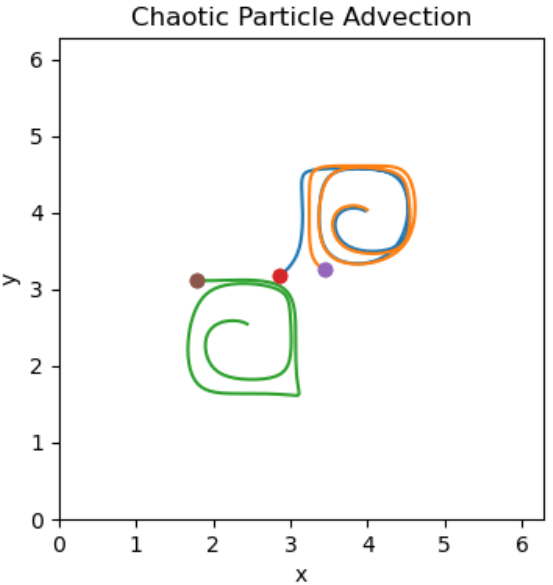
\includegraphics[width=0.8\linewidth]{figures/cellular_flow_advection.png}}
\column{0.5\linewidth}
\begin{figure}
    \centering
    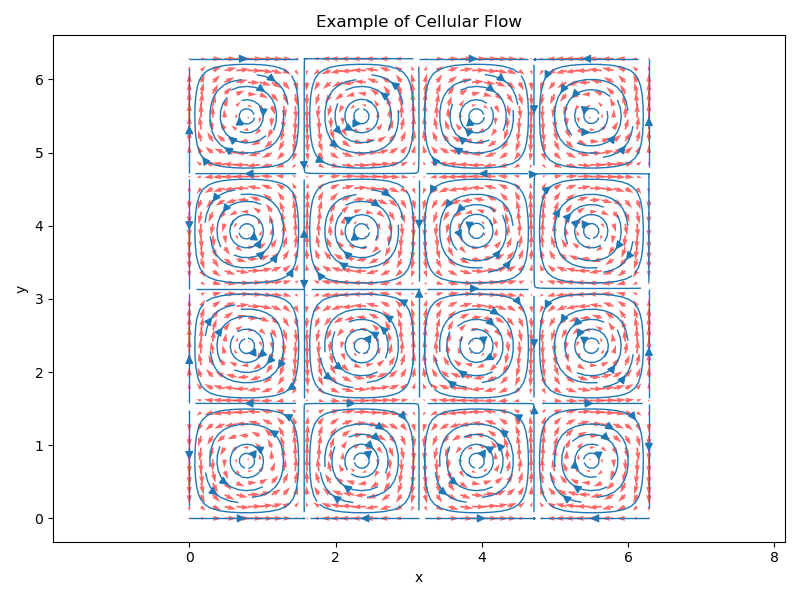
\includegraphics[width=1.2\linewidth]{figures/cellular_flow_field.png}
\end{figure}
\end{columns}
\end{frame}

\subsection{Numerical Advection Tutorial}
\begin{frame}{An advection example in one dimension}

\begin{itemize}
\item {\small{}We model a longitudinal estuary, where the current velocity
is along the $x$ direction and constant; $u=c$ and $v=0$ }{\small\par}
\item {\small{}It's a wide estuary, with homogeneous processes in the meridional
and vertical directions: $\partial_{y}=0$ and $\partial_{z}=0$ for
all properties}{\small\par}
\item {\small{}The vertical depth is too small to generate effective vertical
velocities: $w=0$}{\small\par}
\item {\small{}An initial perturbation of temperature (e.g. hot water leak
from a power plant) occurs at one point in time and over a range of
space. We want to study the evolution of this perturbation, which
is described by the 1D advection equation}{\small\par}
\end{itemize}
\[
\frac{\partial\theta}{\partial t}+c\frac{\partial\theta}{\partial x}=0
\]
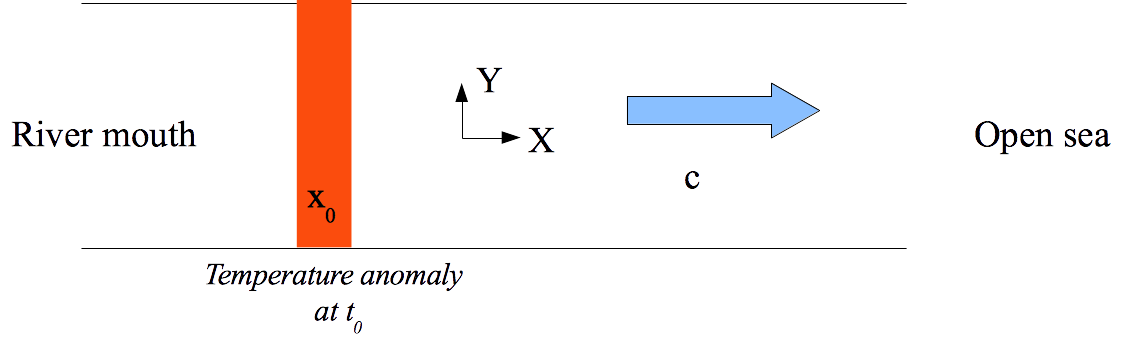
\includegraphics[width=8cm]{figures/river-mouth}
\end{frame}

\begin{frame}{What do we expect?}

The solution we expect is the transport of the perturbation along
the estuary. We are not considering heat exchange or turbulent dissipation,
so the signal will remain undeformed throughout the pathway. This
assumption is not fully realistic but simple to implement codewise

\centering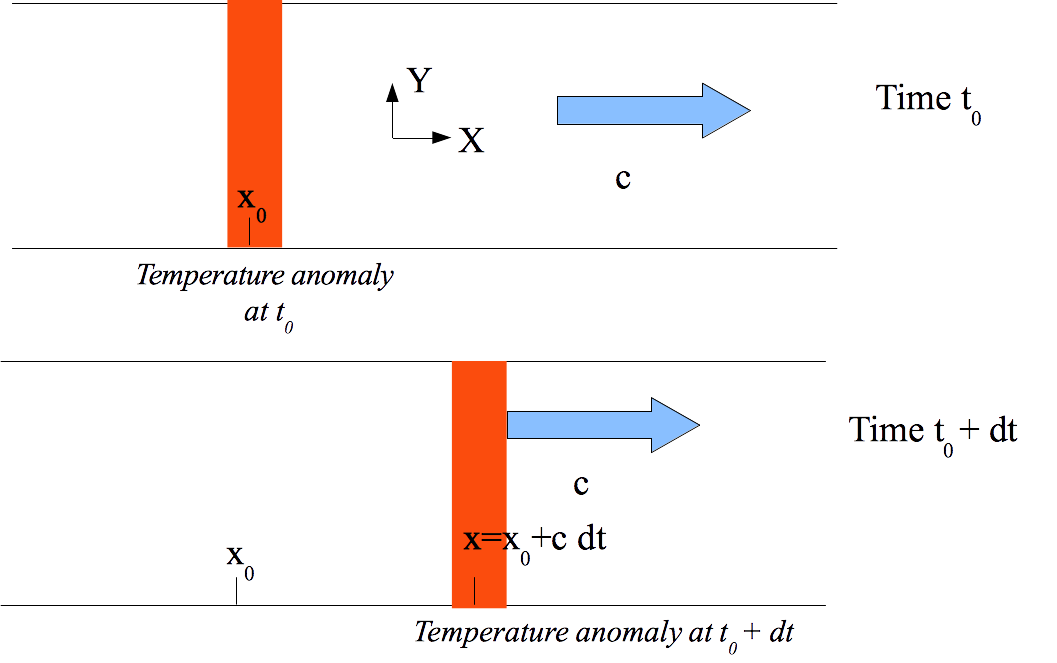
\includegraphics[width=8cm]{figures/river-mouth-evolution}
\end{frame}

\begin{frame}{The expected result shown as a mathematical function}

The solution we expect is the transport of the perturbation along
the estuary. We are not considering heat exchange or dissipation,
so the signal stays undeformed throughout the pathway

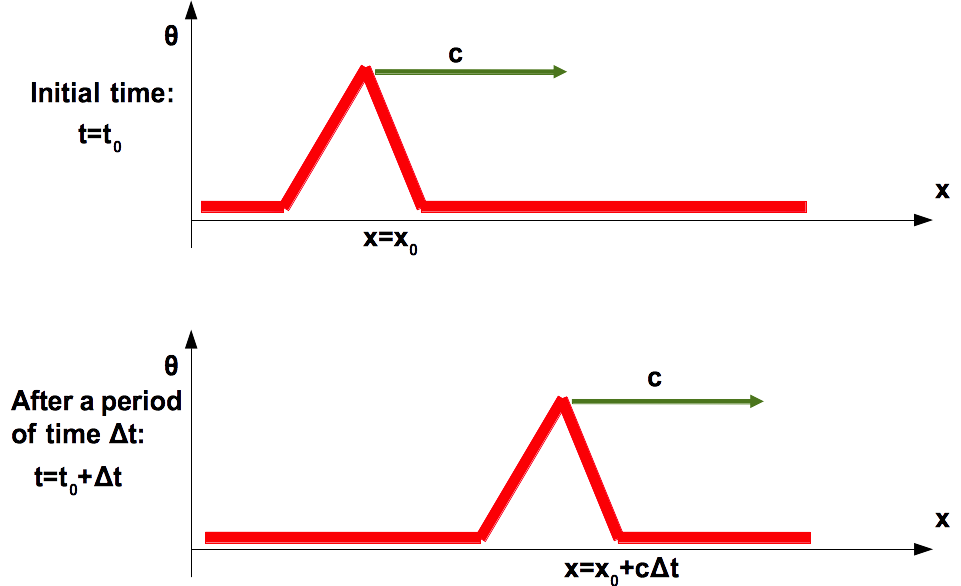
\includegraphics[width=8cm]{figures/wave-advection}
\end{frame}

\begin{frame}{Building the mathematical model}
\begin{columns}[t]
\column{6cm}
\begin{center}
\vspace{-0.5cm}
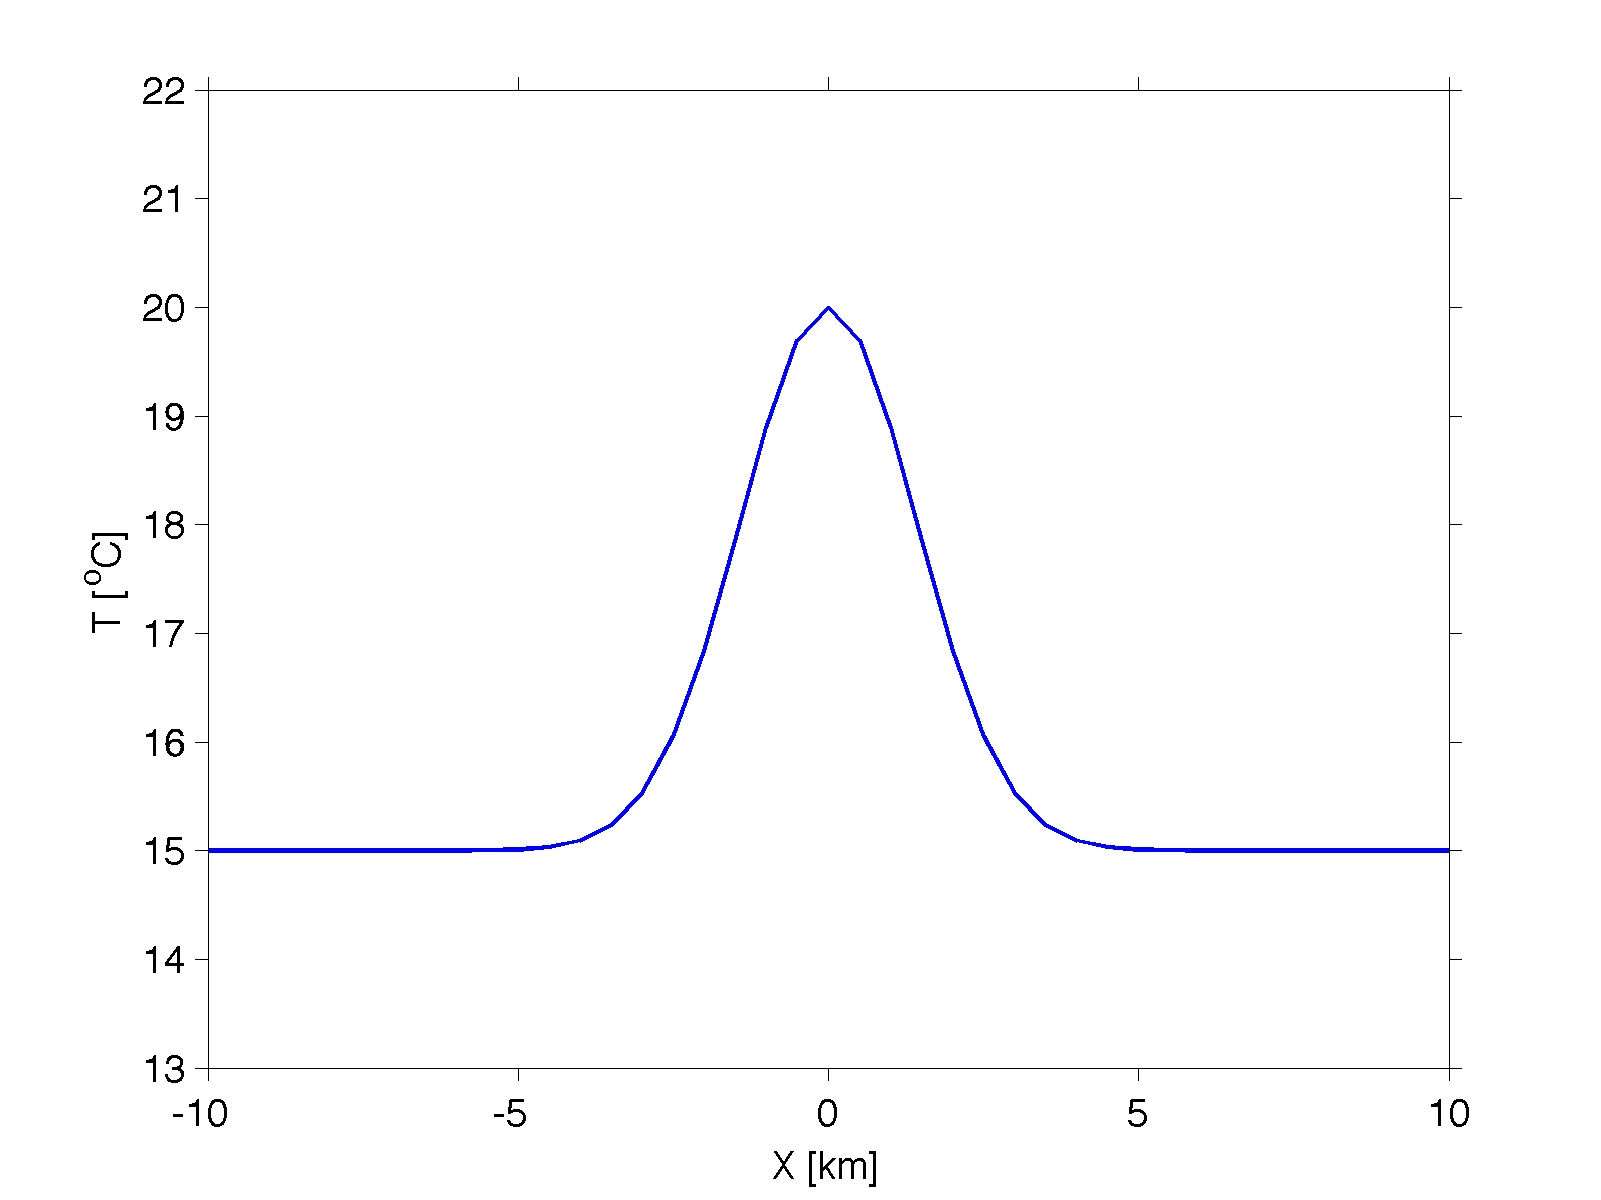
\includegraphics[width=4.5cm]{figures/advection_IC}\vspace{-0.5cm}
\par\end{center}
\begin{center}
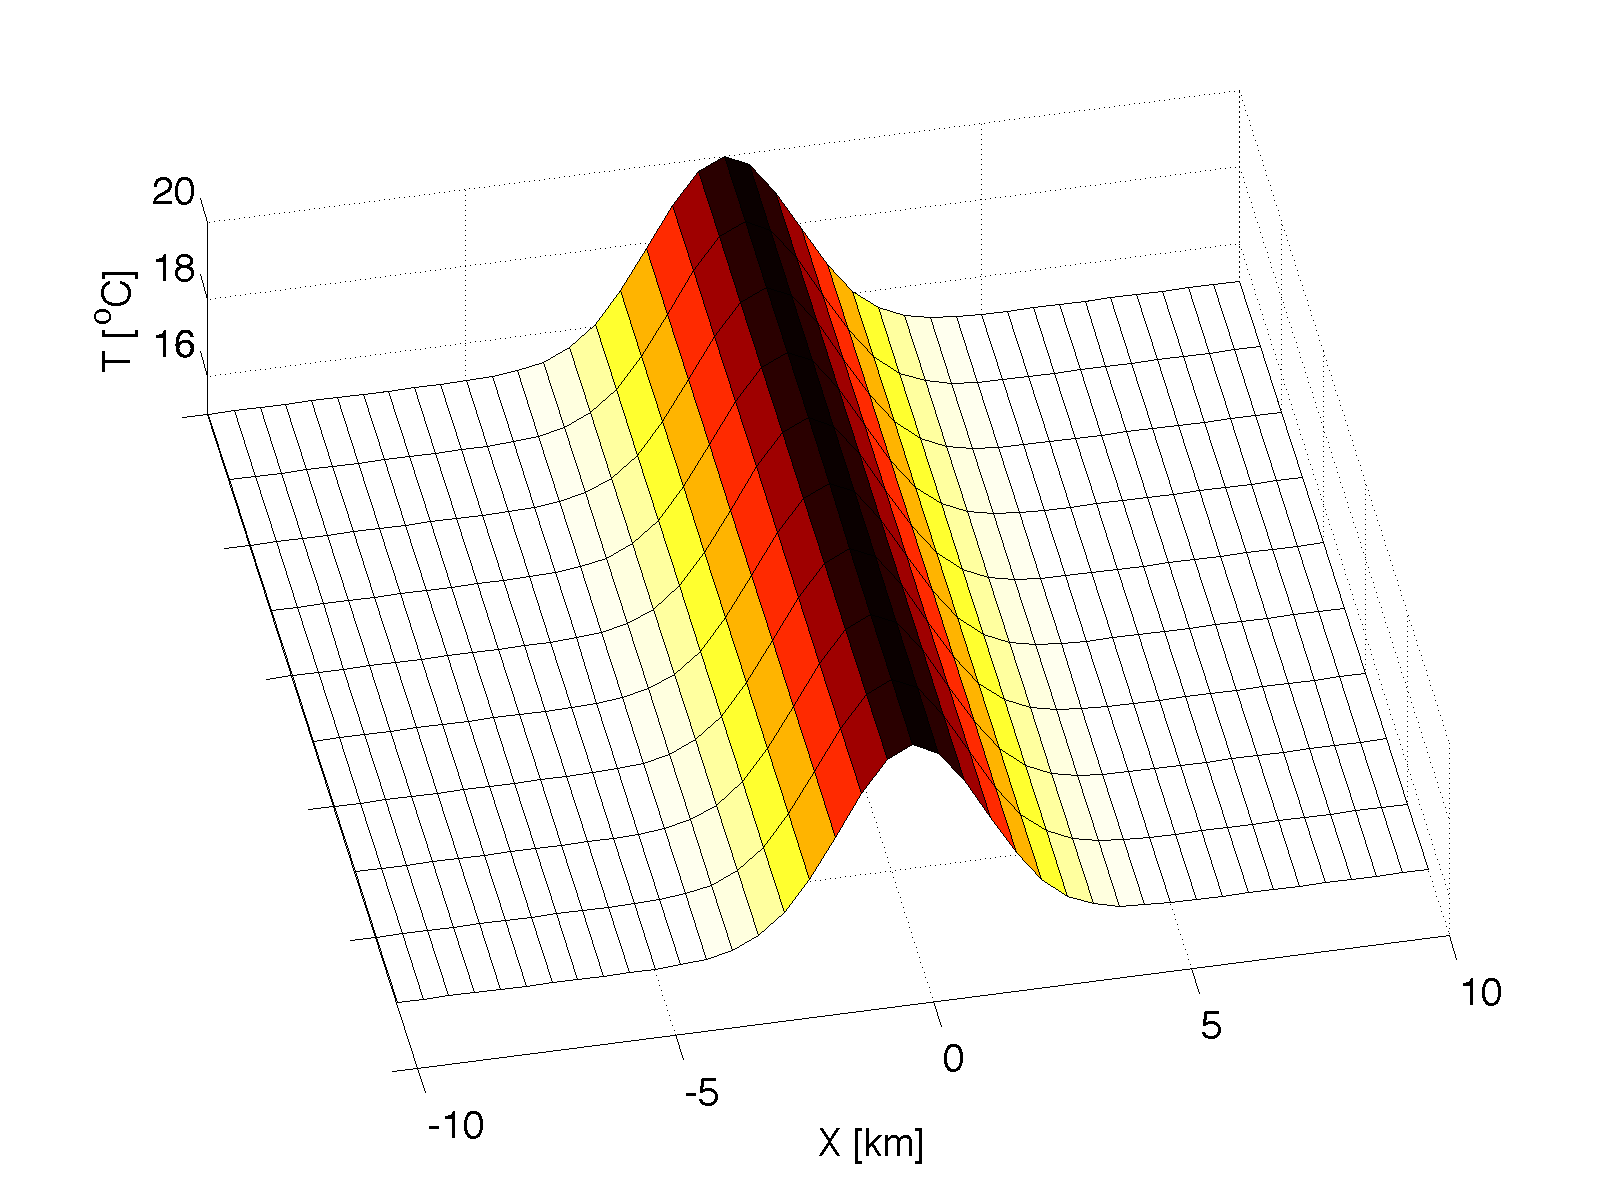
\includegraphics[width=5.5cm]{figures/advection_IC_3D}
\par\end{center}
\column{7cm}
\begin{itemize}
\item {\footnotesize{}For the spatial representation, we choose a channel
of length 20 km and an initial grid step of 500 m. All features are
homogeneous along $y$, so we just need to describe the x-axis}{\footnotesize\par}
\item {\footnotesize{}Our choice for the initial condition function is a
smoothly peaked function, the Gaussian function, that is controlled
by $A$ the amplitude and $\sigma$ the width parameter: 
\[
\theta(t_{0},x)=\theta_{0}+Ae^{-\left(\frac{x}{\sigma}\right)^{2}}
\]
By centering the x-axis around $x_{0}=0$, we get a nicely shaped
perturbation. $x$ is in m, but we are showing km in the plot}{\footnotesize\par}
\end{itemize}
\end{columns}

\end{frame}


\begin{frame}{Exercise US2.4-oce2: display the analytical solution}

\begin{columns}

\column{7cm}
\begin{itemize}
\item Run the following script using python: \texttt{advection\_analytical.py}
(note: this is not a jupyter notebook)
\item Change it into a notebook and show what happens when
\begin{enumerate}
\item you change the values of $dx$ and $c$
\item you increase or decrease the parameter $\sigma$
\end{enumerate}
\item To learn more about animations with matplotlib: \href{https://towardsdatascience.com/animations-with-matplotlib-d96375c5442c}{https://towardsdatascience.com/animations-with-matplotlib-d96375c5442c}
\end{itemize}
\column{6cm}
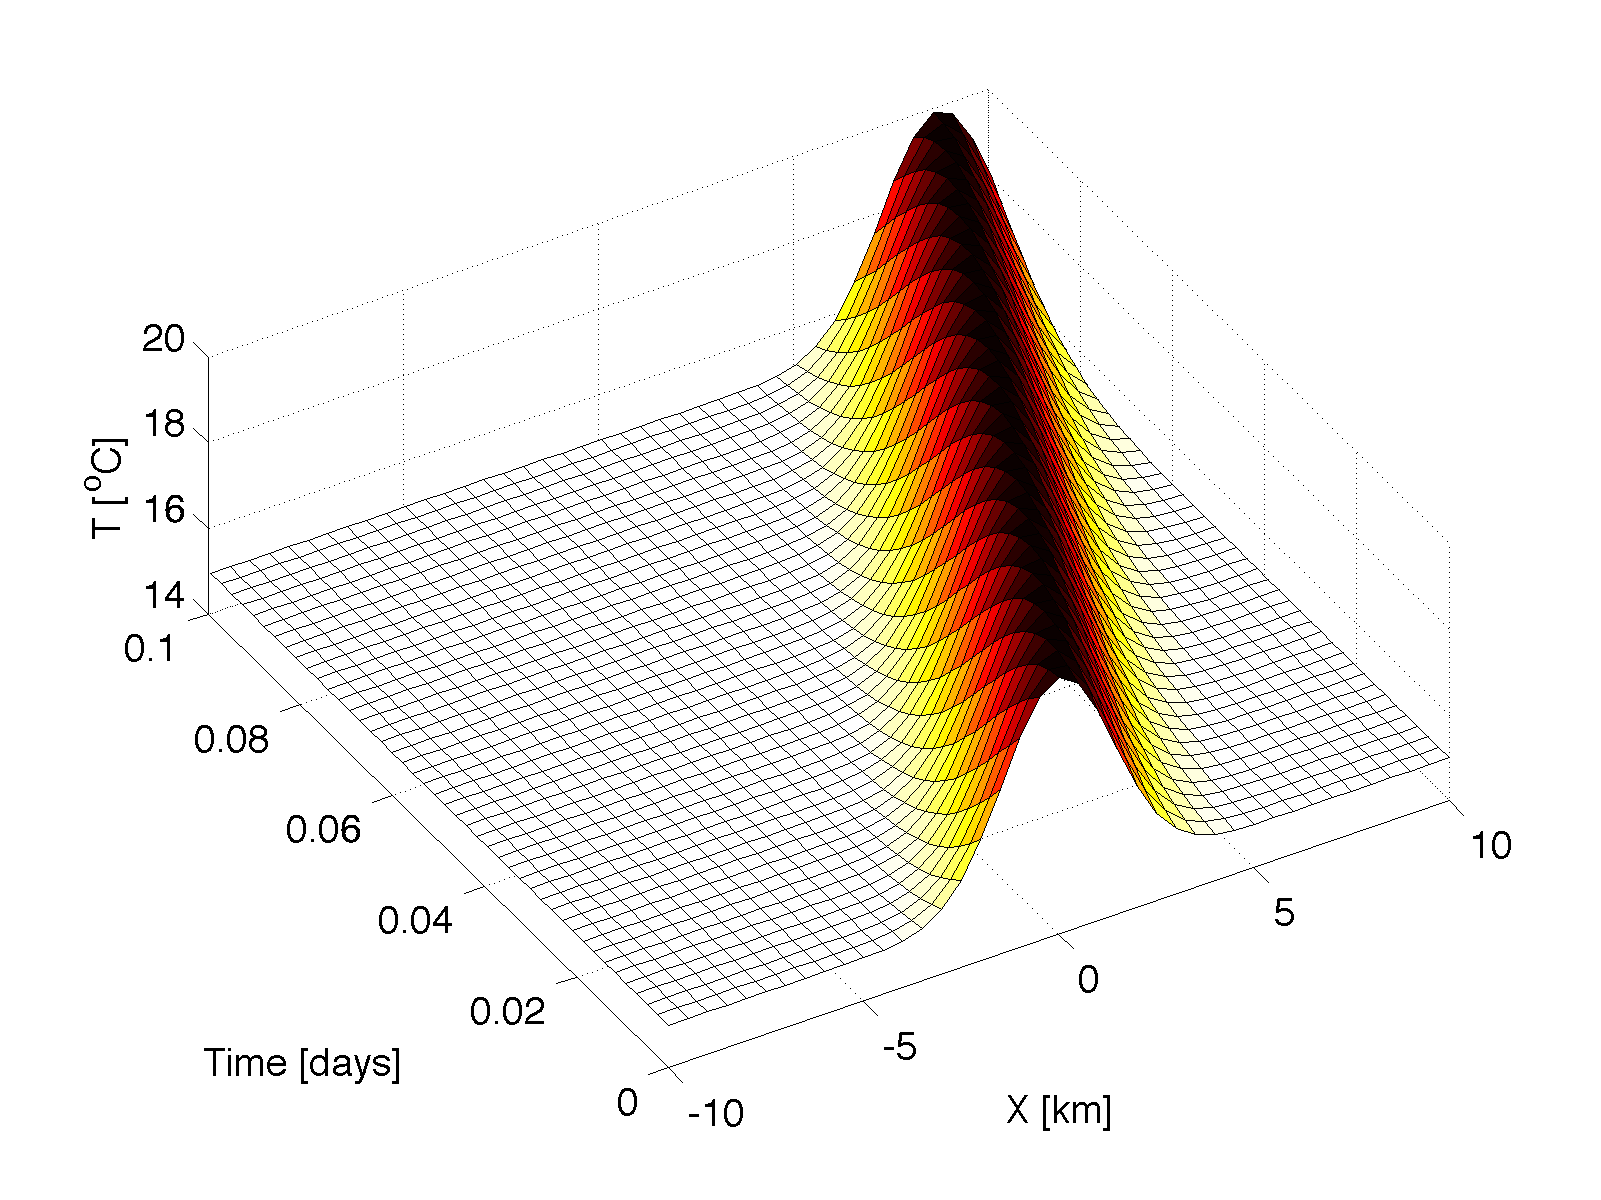
\includegraphics[scale=0.3]{figures/advection_analytical_3D}
\end{columns}
\end{frame}

\begin{frame}{Advanced: The grid for the advection equation\label{fr:advection-grid}}

\begin{center}
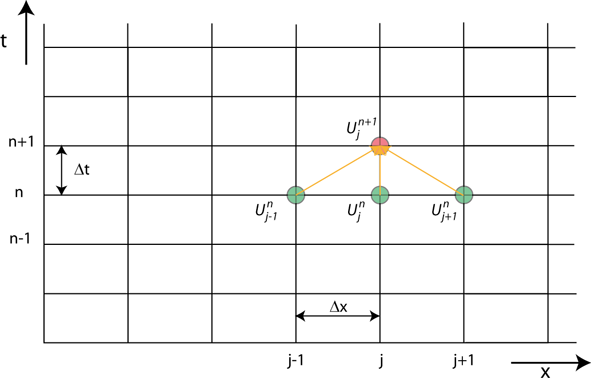
\includegraphics[scale=0.5]{figures/time-space-discretization}
\par\end{center}

{\footnotesize{}This is the stencil that shows how the solution in
time depends on the space variable. A quite natural choice for the
numerical schemes is to use a forward scheme in time and a centered
scheme in space (FTCS). In this example, you should substitute $U$
with our temperature variable $\theta$ and $j$ with $i$ ($i$ is
more natural for indicating the index along the x-axis. We choose
equally spaced points along the $x$ and $t$ dimensions
\[
x_{i}=x_{0}+i\Delta x;\ t_{n}=t_{0}+n\Delta t
\]
}{\footnotesize\par}

{\footnotesize{}and we seek for the solution $\theta_{i}^{n}=\theta\left(x_{i},t_{n}\right)$}{\footnotesize\par}
\end{frame}

\begin{frame}{Advanced: Derivation of the discrete advection equation}

{\footnotesize{}
\begin{equation}
\frac{\partial\theta}{\partial t}+c\frac{\partial\theta}{\partial x}=0
\end{equation}
}{\footnotesize\par}

{\footnotesize{}We have several choices for the derivative term, but
the most obvious way is the explicit Euler forward for time integration
\begin{equation}
\frac{\partial\theta}{\partial t}=\frac{\theta_{i}^{n+1}-\theta_{i}^{n}}{\Delta t}+\mathcal{O}\left(\Delta t\right)\label{eq:adv_FT}
\end{equation}
The advantage of this scheme is that it is explicit: one only needs
the known quantities at time step $n$ to compute the solution at
$n+1$. For the space derivative we use the explicit centered-difference
scheme
\begin{equation}
\frac{\partial\theta}{\partial x}=\frac{\theta_{i+1}^{n}-\theta_{i-1}^{n}}{2\Delta x}+\mathcal{O}\left(\Delta x^{2}\right)\label{eq:adv_CS}
\end{equation}
}{\footnotesize\par}

{\footnotesize{}By combining eqs. \eqref{eq:adv_FT} and \eqref{eq:adv_CS}
we obtain the complete discrete form
\[
\frac{\theta_{i}^{n+1}-\theta_{i}^{n}}{\Delta t}=-c\frac{\theta_{i+1}^{n}-\theta_{i-1}^{n}}{2\Delta x}
\]
which can be rearranged to get the forward-in-time value $\theta_{i}^{n+1}$
\[
\theta_{i}^{n+1}=\theta_{i}^{n}-c\frac{\theta_{i+1}^{n}-\theta_{i-1}^{n}}{2\Delta x}\Delta t
\]
}{\footnotesize\par}
\end{frame}

\begin{frame}{A basic algorithm for the numerical scheme}

\centering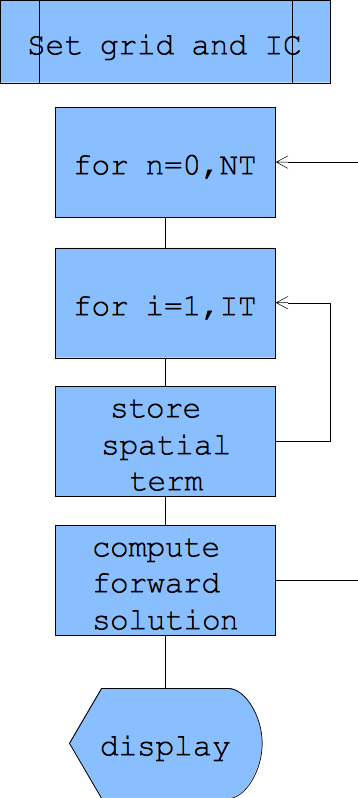
\includegraphics[height=0.8\paperheight]{figures/advection_algorithm}
\end{frame}

\begin{frame}{Is that all?}

\begin{itemize}
\item One may think that by having the algorithm, we now have all the ingredients
to go to the computer room, code it and get a \textquotedblleft good
solution\textquotedblright . And, obviously, the computer will give
some results if we implement the previous algorithm...
\end{itemize}
\begin{enumerate}
\item Is the code efficient or does just work?
\item Will our numerical solution be meaningful? $\Longrightarrow$ Convergence
\item Can we improve it by choosing other finite difference schemes for
our partial derivatives? $\Longrightarrow$ Consistency - Order and
accuracy
\item How can we choose values for $\Delta x$ and $\Delta t$? $\Longrightarrow$
Stability analysis 
\end{enumerate}
\end{frame}


\begin{frame}{Tutorial}

\small{The numerical solution of the advection problem is implemented
in the notebook \texttt{advection.ipynb}.}
\begin{enumerate}
\item {\tiny{}Analysis of the numerical solution. How different is the numerical
solution from the expected moving perturbation? What is the possible
reason?}{\tiny\par}
\item {\tiny{}The grid parameters determine the stability of the solution (called the CFL condition or Courant number, which must be small). The spatial and temporal steps are linked. More spatial resolution (smaller $dx$) means that $dt$ must also decrease to maintain stability. However, things are
not so simple. The higher spatial resolution also enhance the capability to resolve
the real gradients. We will increase the Courant number to 1 by halving $dx$ to check what happens. We will then set $dx=500$ m and $dt=100$ s to get a small Courant number, which means a more stable numerical solution}
\item {\tiny{}The choice of the grid parameters also depend on the features
that you want to resolve. Set the parameter $\sigma=1000$ m (a steeper
wave). What do you have to do to recover the same degree of accuracy
of the previous solution? (note that it takes longer to generate the
movie when you decrease the time step because NT increases and more
frames are generated). Finally, we will double the current speed. How would you explain the results?}
\end{enumerate}
\end{frame}

%-------------------------------------------------
\section{It's a wrap...}
%-------------------------------------------------
\begin{frame}{Real Example: Agulhas Current (Advection and Dispersion)}
\begin{itemize}
\item One of the fastest western boundary currents
\item Transports heat, salt and plankton southward
\item Organisms can be advected large distances and trapped in eddies
\end{itemize}

\begin{block}{Interpretation}
Physical transport directly affects biological distribution.
\end{block}
\end{frame}

%-------------------------------------------------
\begin{frame}{Real Example: Benguela Upwelling (Vertical Mixing + Advection)}
\begin{itemize}
\item Coastal winds drive upwelling
\item Deep, nutrient-rich water rises to the surface
\item Land-see breeze and internal waves increase vertical mixing
\item Fuels high biological productivity
\end{itemize}

\begin{block}{Interpretation}
Vertical transport + mixing control primary production.
\end{block}
\end{frame}

%-------------------------------------------------
\begin{frame}{From Equations to Ecosystems}
\begin{columns}
\column{0.45\textwidth}
\textbf{Physics (equation)}
\[
\frac{\partial T}{\partial t} + u \frac{\partial T}{\partial x} = \kappa \frac{\partial^2 T}{\partial x^2}
\]
\vspace{0.3cm}
\textbf{Meaning}
\begin{itemize}
\item $u$: transport (currents)
\item $\kappa$: mixing (turbulence)
\end{itemize}
\column{0.55\textwidth}
\textbf{Ecosystem impact}
\begin{itemize}
\item Plankton patches are transported by currents
\item Nutrients are mixed upward from depth
\item Spatial patterns of productivity emerge
\end{itemize}
\vspace{0.3cm}
\textbf{Examples}
\begin{itemize}
\item Agulhas: fast advection redistributes organisms
\item Benguela: mixing + upwelling fuels blooms
\end{itemize}
\end{columns}
\end{frame}
%-------------------------------------------------
\begin{frame}{Why Models Are Imperfect}
\begin{itemize}
\item Equations are approximations
\item Grid resolution is limited
\item Some processes are not fully understood
\end{itemize}

\begin{block}{Take-home}
Models are tools to understand the ocean, not exact reality.
\end{block}
\end{frame}

%-------------------------------------------------
\begin{frame}{Applications in Marine Ecosystems}
\begin{itemize}
\item Predicting phytoplankton blooms
\item Understanding larval transport
\item Studying hypoxia
\item Ocean carbon cycle
\end{itemize}
\end{frame}

%-------------------------------------------------
\begin{frame}{Key Takeaways}
\begin{itemize}
\item Ocean models solve physical balance equations
\item Continuous equations are solved on discrete grids
\item Advection and diffusion are core processes
\item Resolution and parameterization are critical
\end{itemize}
\end{frame}

\end{document}
